%----------------------------------------------------------------------------------------
%	CHAPTER 4
%----------------------------------------------------------------------------------------

\chapter{METHODOLOGY}

In this chapter, we show the methods we employ to create our proposed thesis solution to the long latency bottleneck satellite link problem described in previous chapters. 

\section{Socket Programming In C}
Our proposed solution to the stated research problem involves the design of a performance enhancing proxy (PEP) modified to suit the Pacific Island environment. The novelty or distinguishing facets/distinctive qualities of our PEP will be elaborated on in Section 4.3 "Our Proposed Solution", but we first start with the discussion of a few techniques that are specific to the type of programming used for standard PEP creation; namely raw socket programming. There are other languages we could have chosen to use for Socket programming (Java, Python) but we chose to use C as it is one of the few languages that properly supports raw sockets and is also the fastest once compiled. Fast processing speed is important in the satellite type environment ~\cite{35}.\\

C is ideal for firmware or portable applications. Its proximity to assembly language means that although it is considered a high-level language,  it is low level enough by comparison to modern language standards (C\#, Java, Python) to allow detailed composition, manipulation and parsing of Internet packet structures ~\cite{35}~\cite{36}. This feature is essential because to create the PEP, we must be able to spoof packets and resend them, and this will involve reading incoming packets and resetting flags and ACKs, creating our own ARP packets and more to emulate expected responses to and from two different hosts in the network. These actions require access to the IP layer, TCP transport layer and the data link layers. We will need raw socket programming for this purpose ~\cite{38}. 

\subsection{Sockets}
\begin{figure}[h!]
    \centering
    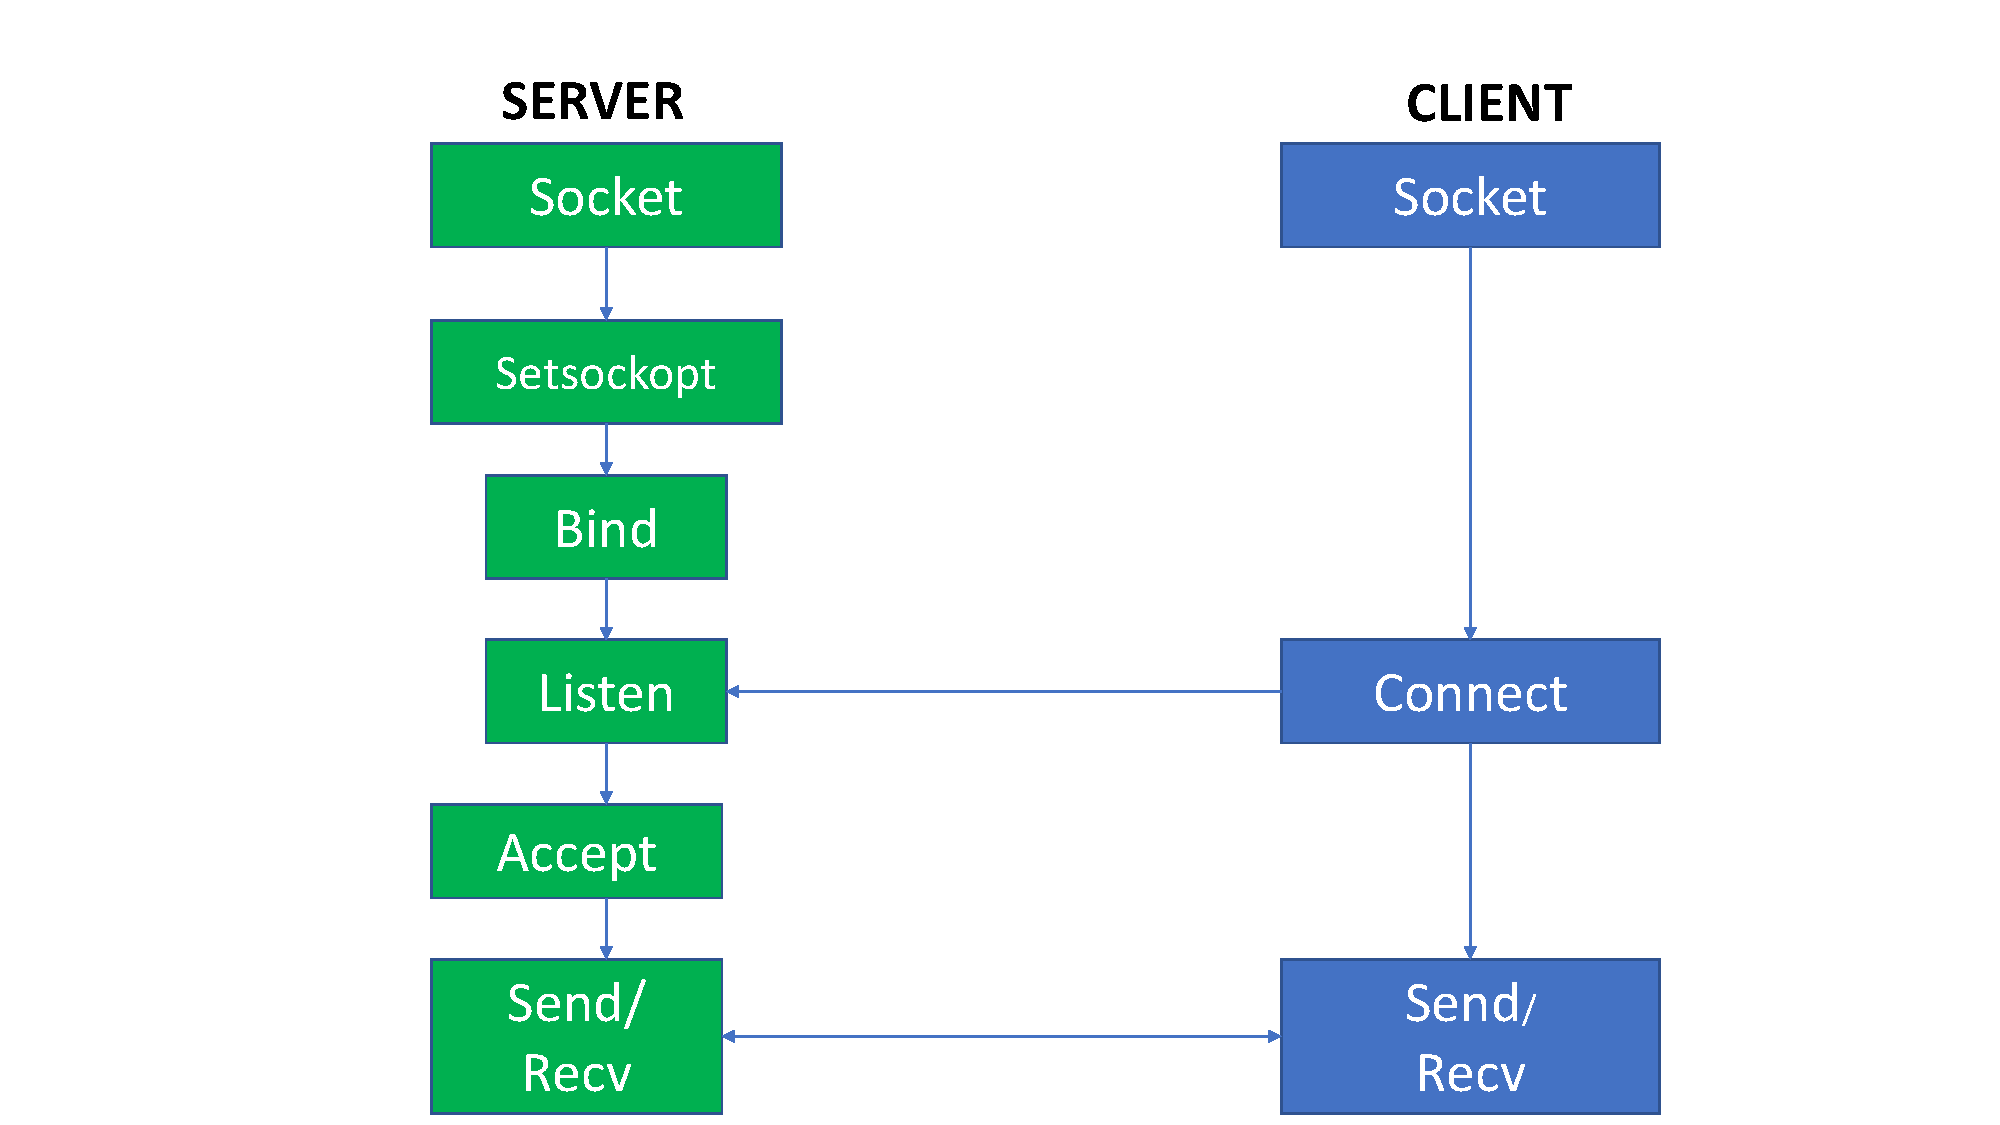
\includegraphics[width=1.2\textwidth]{ServerClient.pdf}
    \caption{Server + Client Sockets. Shows interaction between Server and Client via Sockets.}
    \label{ServerClientModel}
\end{figure}

Sockets are a key concept for this thesis. This thesis, however, will be dealing with raw sockets but to understand what raw sockets are, we must first understand what sockets are in general, of which raw sockets are a subset ~\cite{38}. In C, raw sockets are available for use at the transport layer (TCP), IP layer and data link layers. The following example described below are for the more commonly used transport layer sockets. \\

Sockets are endpoints for communication in the network infrastructure. They allow two nodes in a network to communicate with one another. Without getting too technical, the socket concept can be understood, in simple terms, using a telephone analogy. When we create the sockets via socket programming, it is analogous to installing a telephone on either end of the communication line between two parties ~\cite{37}. The telephone/socket is an endpoint between two parties/computers that enables them to establish communication. An endpoint is a unique combination of an IP address and a port number in the networking world. The telephone can be likened to an endpoint combination of a telephone number (IP address) and an extension number(port number) ~\cite{37}. \\

In the network world, the Client-Server model is the basis for most communication. The Server is always listening for a client to connect. Once a client connects after connection handshake, it can request information. The Server serves this information to the client and the client disconnects (the server can also disconnect). The Server will be on standby again to listen for more connections from clients ~\cite{35}. \\

We can create sockets using a few "function calls" or set of programming requests from the socket application programming interface/ socket API. In keeping with the telephone analogy, here are a few of the key code calls used in socket programming in C ~\cite{35}~\cite{36}.
   \begin{itemize}
   \item Socket() -Endpoint for communication/ create telephone on either end:\\
   int socket = socket(domain, type, protocol)
   \item Bind()- Assign a unique IP address and specific port number/ telephone number to distinguish this endpoint from other endpoints on the network:\\
   int bind(int socket, const struct sockaddr *addr, 
                          socklen\textunderscore t addrlen);
   \item Listen()- Listen for an incoming connection/ wait/be ready for an incoming call:\\
   int listen(int socket, int backlog);
   \item Connect() -request connection to another endpoint/ dial a phone number:\\
   int connect(int socket, const struct sockaddr *addr,  
                             socklen\textunderscore t addrlen);
   \item Accept() -accept incoming connection request/ receive a phone call, i.e. answer the phone:\\
   int new\textunderscore socket= accept(int socket, struct sockaddr *addr, socklen\textunderscore t *addrlen);
   \item Send(), Recv()- exchange data over the established connection/ talk over the phone to the other person: \\
   ssize\textunderscore t send(int socket, const void *buf, size\textunderscore t len, int flags);
   ssize\textunderscore t recv(int socket, void *buf, size\textunderscore t len, int flags);
   \item Close()- Terminate connection and endpoints/ hang up the call once talking is done. \\
   int close(int socket);
   \end{itemize} 
   
\noindent \emph{Note: The calls to pay most attention to here for future reference are {\tt Socket(), Bind(), Send()} and {\tt Recv()} as they will be used again in raw socket programming for the PEP.} 

\subsubsection{Regular TCP sockets vs raw sockets}
Regular socket programming operates on the transport layer protocol. It deals with TCP and UDP transmission taking in byte stream data as input to form TCP segments. Regular TCP sockets take care of encapsulating TCP segments (including TCP headers, checksums etc.) in IP datagrams (including IP headers and header checksums) but do not alter or touch the contents of the packets which are handled by the kernel operating system. Hence the following operations are also automatically handled in regular TCP sockets ~\cite{35}:\\

\begin{itemize}
\item Ensures ACKs, retransmission, flow control, congestion control for TCP, datagrams etc.
\item Ensures encapsulation of IP datagrams into physical layer frames (typically Ethernet) including frame headers and checksums.
\item Ensures reassembly of IP datagrams from frames + fragments
\item Extraction of TCP segments
\item Ensures completeness of byte stream from TCP segments
\item outputs byte stream \\
\end{itemize}

Essentially, automatic encapsulation of the packets with the protocol headers (UDP or TCP) occurs, and the socket-user does not deal with these headers at all. With Raw Sockets, many of these operations mentioned are not handled automatically and must be programmed manually. Raw sockets are aware of the packet headers in that they receive \emph{raw packets} that can include IP headers and/or Ethernet headers depending on whether we are using a network layer or data link layer raw socket. The raw sockets can opt to include or exclude the headers upon transmission. Raw sockets bypasses the standard stack traversal and reaches down into the network and data-link layers to allow us to alter the content of these packet headers ~\cite{35}~\cite{38}.\\

This concludes the general overview, in layman's terms, of what sockets are, their purpose, and how they function.  We are now ready to proceed with explaining the concept of raw sockets in more detail and how it relates to this thesis.\\

\section{Raw Socket Programming}
Raw Sockets enable us to deliver a raw packet directly to an application without it traversing through the stack of network layers (See Figure 4.5).
In other words, we can circumvent the usual TCP/IP protocols, and this enables us to create a packet sniffer and packet injector to modify packets as per requirements for our specialised PEP ~\cite{38}. \\

\textbf{Raw sockets allow the following:}\\

\begin{enumerate}
\item Inject IP packets directly into Ethernet frames (but let the kernel take care of Ethernet frame assembly) and send them.
\item Assemble and send entire Ethernet frames
\item Receive Ethernet frames/IP packets individually regardless of protocol\\
\end{enumerate}

The network stack removes all headers from packets as they move up the stack, transporting only the data to the application layer. (See Fig 4.3). Conversely, data sent from the application layer back the other way has headers added as it traverses down the stack. So whilst other sockets only interact with the transport layer and deal exclusively with payload data, raw sockets take packets from the Ethernet layer(raw packets) complete with headers and can forward them directly to the intended application. If a communication flow is occurring between different processes in regular sockets, then these processes are only exchanging data ~\cite{38}.\\

Raw packets, defined as a packet with headers included, have the source IP address and MAC address information loaded into their headers, and this is crucial information needed to construct our PEP. Our PEP must be able to spoof packet header information in outgoing packets header and forward them to the intended hosts. For this purpose, it must also be able to read IP/TCP headerand Ethernet header information. The next section will detail how we use raw socket programming to build our PEP starting with a fundamental building block for all PEPS: \emph{The packet sniffer} ~\cite{38}.\\

\begin{figure}[h!]
    \centering
    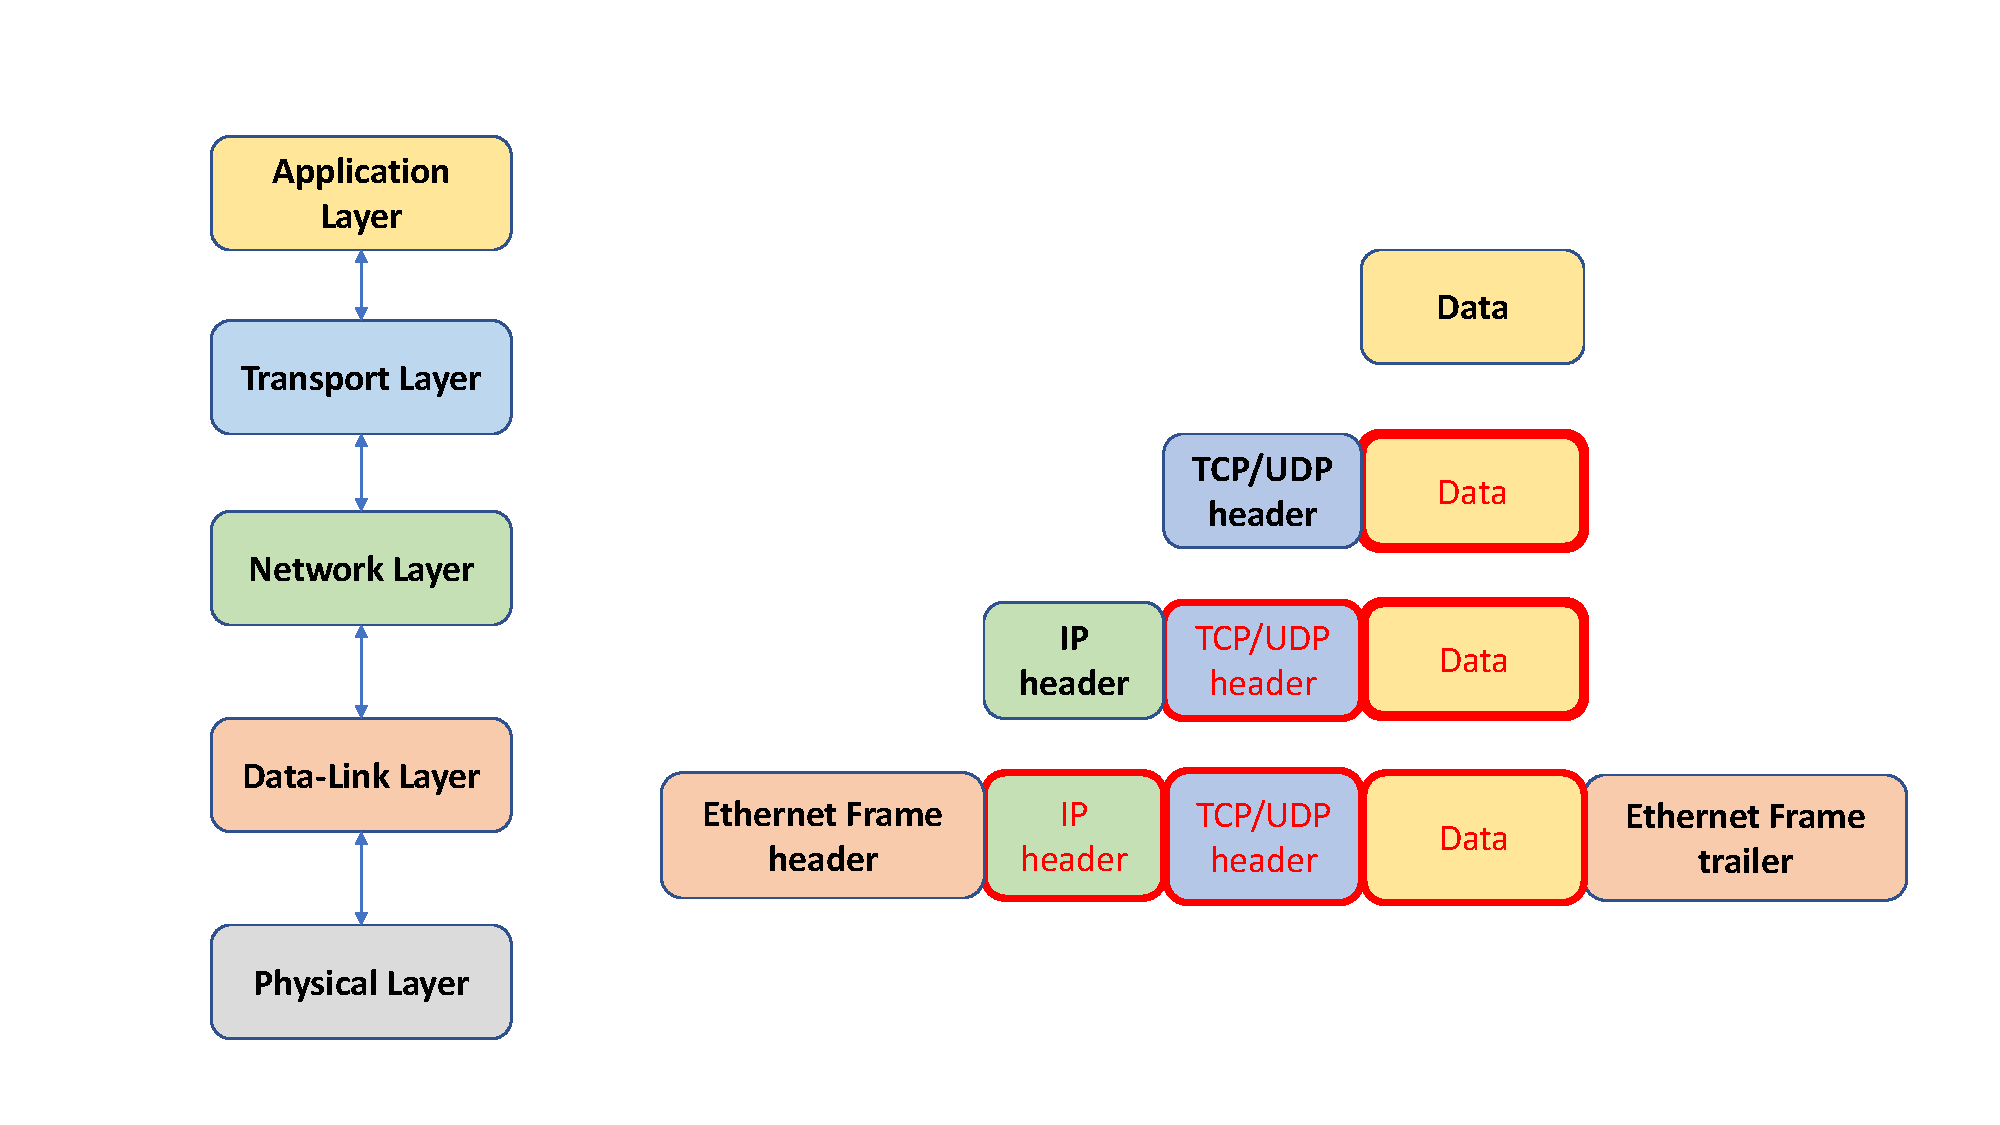
\includegraphics[width=0.95\textwidth]{NetworkTraversal.pdf}
    \caption{Headers being stripped + added during Network Stack Traversal
    }
    \label{fig:Socket}
\end{figure}

\subsection{Creating a packet sniffer}
To build a PEP that can forward packets and that can act as a proxy that can emulate ACKs for incoming packets, we need to be able to intercept and fully interpret these packets. The PEP must be able to see all the information in the headers as well as the data payload. This requires the creation of a packet sniffer as the first step to achieving our PEP ~\cite{38}. \\

We are using a Linux system for experiments in the lab. Linux has its own packet sniffer tool called \textbf{tcpdump} ~\cite{35}, but for this thesis we created our own packet sniffer with C programming. This provides one of the building blocks for our non-connection breaking PEP. \\

\textbf{To create a packet sniffer, we first need to create a raw socket:} \\

The packet sniffer is created by: 
    \begin{itemize}
        \item Using raw socket call to create a socket object- \\
        {\tt int socket= socket(int socket\textunderscore family, int socket\textunderscore type, int protocol);}\\
{\tt \textbf{rawSocket = socket(\textcolor{blue}{AF\textunderscore INET}, \textcolor{purple}{SOCK\textunderscore RAW} , \textcolor{orange}{IPPROTO\textunderscore TCP});}}
        \item Make sure interface is set to promiscuous mode for packet sniffing. Allows us to receive all packets, not just packets bound for the machine attached to the interface- use {\tt ioctl()} or use infinite while loop with {\tt recv()} (See Figure 4.4 for an example).
        
        \item Bind Raw Socket to the interface we want to listen to-use {\tt bind()}\\
{\tt int bind(int socket, const struct sockaddr *addr, socklen\textunderscore t addrlen);}\\
{\tt \textbf{bind(sd, (\textcolor{purple}{struct sockaddr *}) \&sll, \textcolor{blue}{sizeof}(sll))) == -1)}}
\item Receive packets on the socket using recv()\\
{\tt recv(int sockfd, void *buf, size\textunderscore t len, int flags);}\\
{ \tt \textbf{recv(rawSocket, buffer,\textcolor{blue}{65536}, 0)}}

        \item Close the raw socket() -never reaches this point if on infinite while loop\\
        int close(int rawSocket);\\
    \end{itemize}
    
The packet sniffer will set the interface to promiscuous mode so that it receives frames for all hosts in its broadcast domain irrespective of whom they are addressed to. Simply put, the sniffer allows eavesdropping on all packets observed on the same physical network ~\cite{35}~\cite{38}.\\

The sniffer will receive raw packets, complete with TCP, IP and Ethernet headers, or ARP headers, ICMP headers etc., for example, which we will be able to analyse and manipulate via our PEP. The next step component for the PEP is the capability to inject packets into the network. Once our PEP has analysed the sniffed packet and extracted the data, we can manufacture our own spoofed packets with custom-made headers and data payload for forwarding ~\cite{38}.\\

\subsection{Creating a packet injector}
Another essential element in the creation of our PEP is the ability to forward incoming packets the PEP receives.  
The creation of the packet injector is similar to that of the set up for a packet sniffer ~\cite{35}~\cite{38}.  \\

\textbf{For packet injector-}\\
    \begin{itemize}
        \item Using raw socket call to create a socket -socket()
        \item Bind Raw Socket to the interface we want to send packets on-use bind() or setsockopt()
        \item Create a new packet using info extracted from the sniffed packet
        \item Send the packet -sendto() transmits the packet to another socket \\
sendto(int socket, const void *buf, size\textunderscore t len, int flags,
               const struct sockaddr *dest\textunderscore addr, socklen\textunderscore t addrlen);        
        \item Close the raw socket()\\
    \end{itemize}

\begin{figure}[h!]
    \centering
    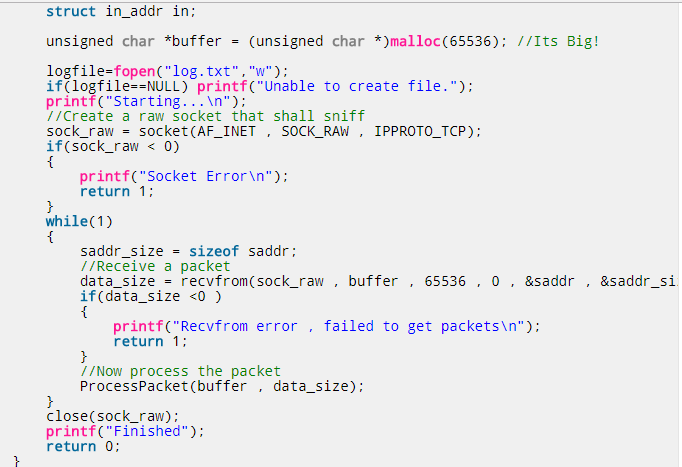
\includegraphics[width=0.87\textwidth]{SnifferCode.PNG}
    \caption{Example of basic sniffer code in Cl
    }
    \label{fig:Sniffer code in C}
\end{figure}

The sample code in Fig 4.4 shows the basic setup for a sniffer. We see the socket () call taking three parameters, int domain, int type and int protocol which returns an int that represents a socket file handle of the operating system ~\cite{35}~\cite{38}. \\

The \textbf{domain} here is AF\textunderscore NET which stands for "Address Family", and this allows for IP addresses specifically. 
A socket address in the AF\textunderscore INET family contains four fields: 

\begin{enumerate}
     \item The name of the address family itself (AF\textunderscore INET).
     \item The IP address (Ipv4).
     \item The port number.
     \item The reserved field of 8 bytes ~\cite{36}. \\
\end{enumerate}

The \textbf{type} specifies the type of socket we want to open. For regular socket programming, we want to open either a SOCK\textunderscore STREAM for a TCP socket or SOCK \textunderscore DGRAM for a UDP socket. For the packet sniffer, we require a raw socket that receives full packets (raw packets) with header information (Source IP, Source MAC address etc.) included, so we use the constant parameter SOCK \textunderscore RAW as  \textbf{type} ~\cite{36}~\cite{38}. \\

Lastly, we have the \textbf{protocol} parameter which is set to IPPROTO\textunderscore TCP in the code snippet (Figure 4.4) which sets up the sniffer to receive raw TCP packets. Usually, only one protocol exists within a socket so it can be set to 0 but in some cases, there is more than one, so the need to specify a protocol is required ~\cite{35}.\\

\begin{figure}[h!]
    \centering
    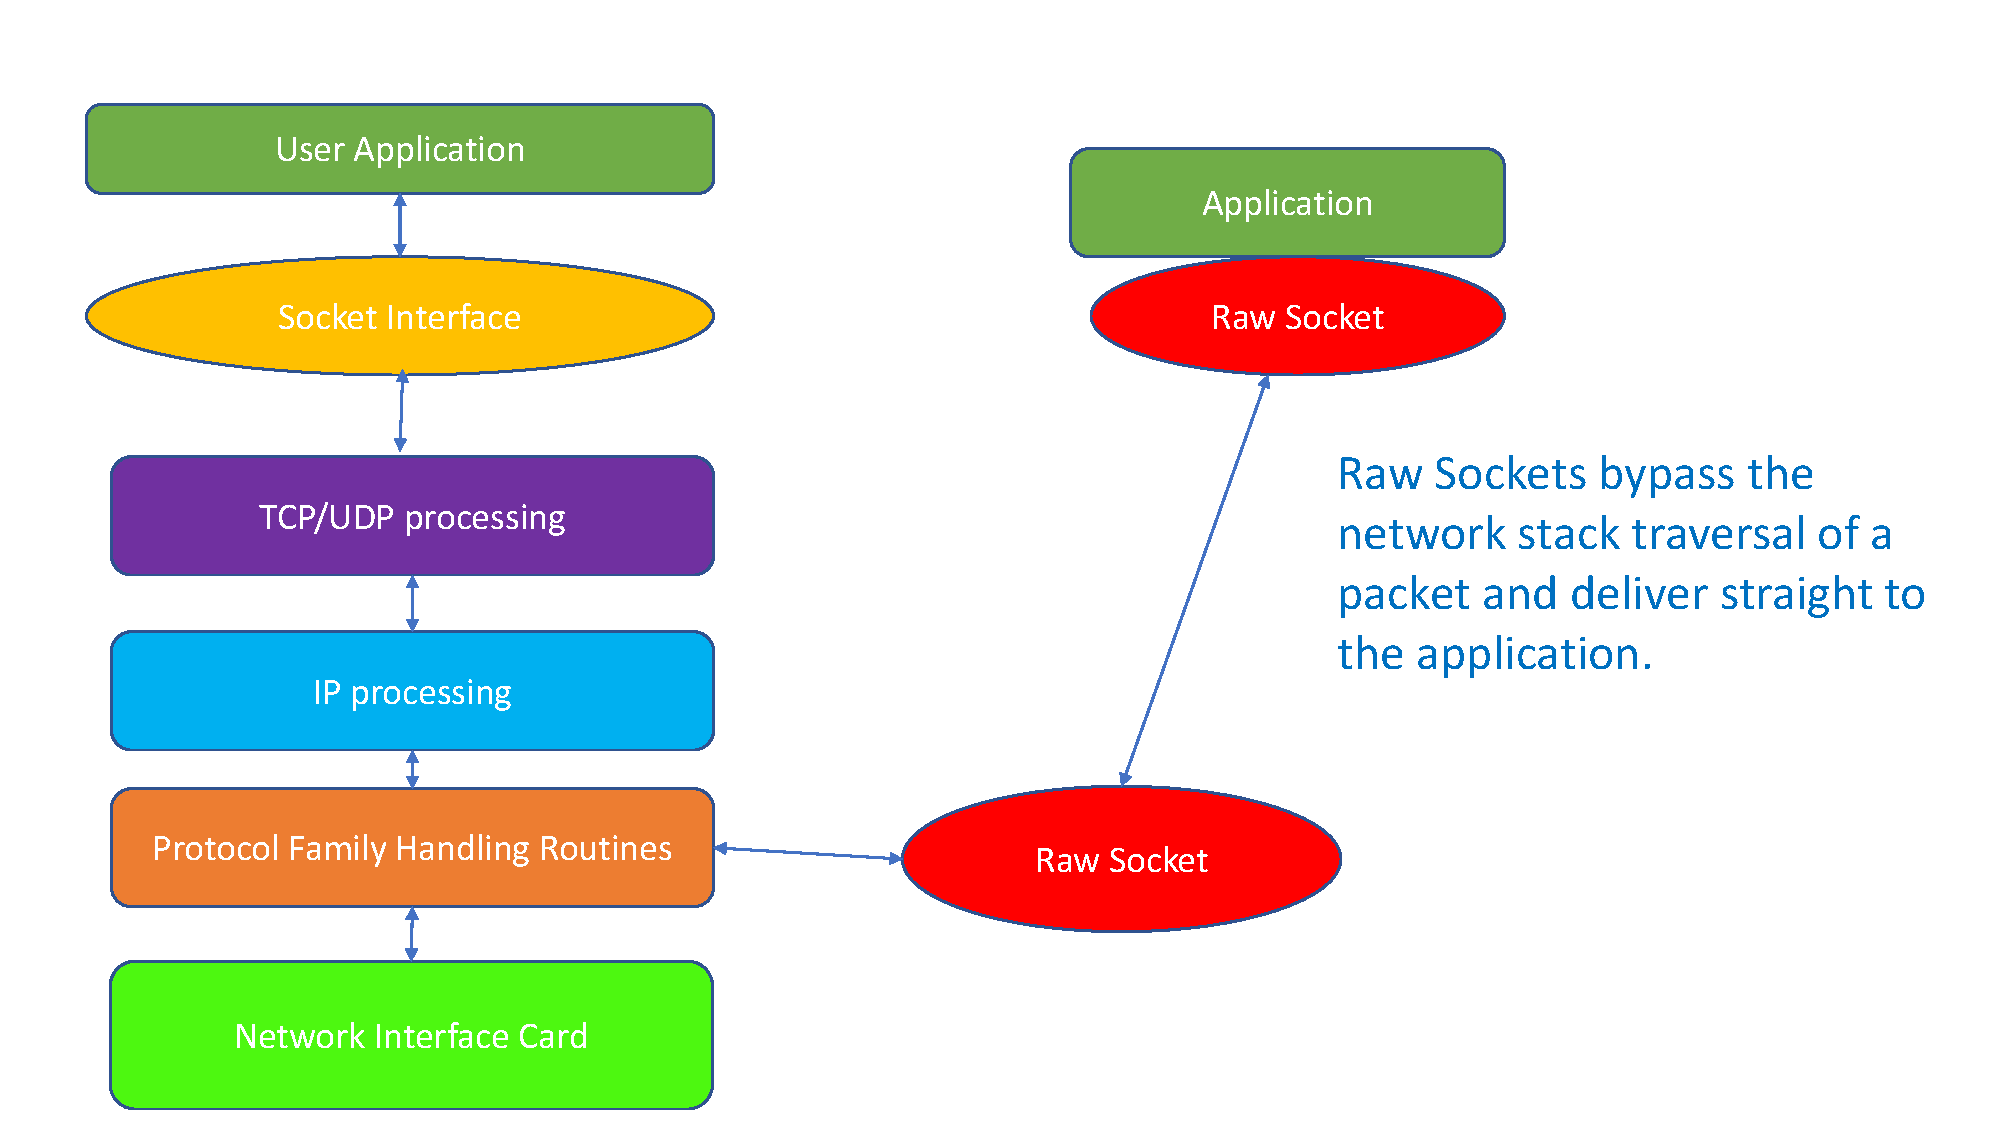
\includegraphics[width=0.95\textwidth]{stackTraversal.pdf}
    \caption{Raw Socket Bypassing Kernel Stack Traversal}
    \label{RawSocketTraversal}
\end{figure}

We also have IPPROTO\textunderscore IP, if used in conjunction with socket type SOCK\textunderscore STREAM and AF\textunderscore NET, causes the kernel to set the protocol to TCP automatically (as if using IPPROTO\textunderscore TCP). \\

The same, however, will not work when these two parameters are used with SOCK\textunderscore RAW. The SOCK\textunderscore RAW must be used with the correct protocol which can only be called explicitly ~\cite{36}~\cite{38}.\\

In our sniffer, we set the protocol to IPPROTO\textunderscore RAW as we want to interact directly with the lower layers 3 (network layer) and layer 2 (data-link layer/Ethernet). The prepending of headers is usually handled by the kernel, but we want to execute packet injections from our PEP and edit the headers and payloads ourselves. This gives us the flexibility needed to spoof packets and override any default information from the kernel by bypassing the usual stack traversal processes altogether (see Fig. 4.5) ~\cite{38}.\\

\subsection{Binding sniffer to an interface}
The next step is to bind that sniffer to an interface we want to listen to. Binding the sniffer to a particular interface ensures that the sniffer only listens for packets on the bound interface, rather than on every interface. \\

To do this, we need to extract the interfaces kernel identification number or file handle using standard \emph{ioctl} calls which we will explain in more detail later. \todo{promise}Since we are coding this in C; we are dealing with structs (See Section 2.2.5 - Other Concepts Used In This Thesis). \\

We can liken structs to classes in Java complete with fields or attributes but excluding methods ~\cite{39}. The sniffer code will use structs to store the information needed for various operations. This thesis will not delve into structs in too much detail. Although structs are a concept of C programming that is used here, understanding the struct concept and how it is used to create our PEP is sufficient ~\cite{39}. As can be seen in the struct ifreq below, we see a struct that looks like a class with attribute fields. Structs ifreq in the code snippet 4.6 is declared as struct ifreq {\tt ifr} with {\tt ifr} being a variable of type struct ifreq. \\

Take note of the fields in the struct ifreq below and the caption in figure 4.6 explaining the code attached to the ioctl call. The ioctl call in figure 4.6 will look at the interface name that is stored in the {\tt ifr\textunderscore name} field and returns the interface index number and stores it in the {\tt ifr\textunderscore index} field. \\

\lstset{language=C,
                basicstyle=\ttfamily,
                keywordstyle=\color{blue}\ttfamily,
                stringstyle=\color{red}\ttfamily,
                commentstyle=\color{green}\ttfamily,
                morecomment=[l][\color{magenta}]{\#}
}

\begin{lstlisting}
struct ifreq { 
    char ifr_name[IFNAMSIZ]; // Interface name
    union {
        struct sockaddr ifr_addr;
        struct sockaddr_ifr_dstaddr; 
        struct sockaddr ifr_broadaddr;
        struct sockaddr ifr_netmask;
        struct sockaddr ifr_hwaddr;
        short ifr_flags;
        int index;
        int ifr_metric;
        int ifr_mtu;
        struct ifr_map;
        char ifr_index;
        char sockaddr ifr_metric;
        char sockaddr ifr_mtu;
    };
};
\end{lstlisting}

\begin{figure}[h!] 
    \centering
    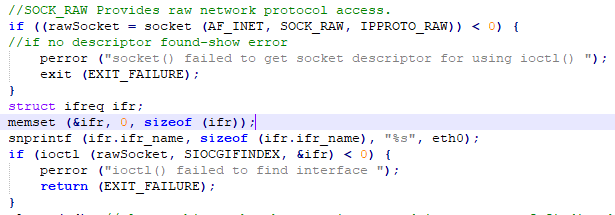
\includegraphics[width=0.9\textwidth]{Struct_ifreq.PNG}
    \caption{IOCTL call to find interface kernel index. ifreq struct {\tt ifr} has been nulled out by memset. The snprintf stores the name of the chosen interface as a string in the {\tt ifr} name field. Next the ioctl takes a rawsocket as its first parameter, uses it to carry out the instruction in the second parameter (SIOGIFINDINDEX) to find the kernel index of the interface name stored in {\tt ifr} name field. Finally, on successful completion, The index number is stored the {\tt ifr} index field}
    \label{fig: http://man7.org/linux/man-pages/man7/netdevice.7.html}
\end{figure}

\subsubsection*{Struct Ifreq:}
For our lab's Linux based systems, we can use a struct ifreq to pass data received via an ioctl call as seen in line 3 of Fig 4.6 {\tt "ioctl(rawSocket, SIOCGIFINDEX, \&ifr)"}. Linux makes use of standard ioctl calls for configuration of network devices ~\cite{40}. They can be utilised in conjunction with any socket file descriptor to retrieve information about the network (e.g. interface name, interface index, interface MAC address etc.). The ioctl call will find the interface name that is stored in the ifreq struct {\tt ifr} and can extract any of the attribute information contained in its struct fields (in this case, we want interface index number as catalogued by the kernel so we can use it later to bind our socket sniffer to that interface). The struct ifreq allows a programmer to get and set network configurations ~\cite{40}. \\

In Fig 4.6, ioctl takes three parameters. The first parameter named rawSocket, is a raw socket we create specifically to find the kernel index number for this interface. (Line 1 of Fig 4.6, opens a raw socket). The second parameter is an instruction for the ioctl to perform. In this case, the instruction is to populate the if\textunderscore index field of the ifreq struct using the interface name we stored in the ifreq struct variable ifr. The third parameter is where the socket stores the found kernel index. More specifically, it is the memory address of the corresponding ifreq struct field containing a kernel index ~\cite{35}~\cite{40}. \\

This struct is used frequently throughout this thesis because of its ability to store all the information needed for our packet injector (i.e. interface index number, interface IP address, interface netmask etc). it will have any of its fields populated depending on the instruction given as a second parameter ~\cite{35}~\cite{40}. This will be of use again when the next hop interface MAC address and index are required to forward packets on for our packet injector. This will be discussed in more detail in Section 4.2.4 "Forwarding Packets".\\
 
In Figure 4.7, the {\tt bind()} call will bind the desired interface for "sniffing" via its kernel index number, which we stored earlier in the ifreq struct, to a raw socket ~\cite{35}~\cite{40}. Now the important thing to note is that any packets that pass through this interface will be heard by our sniffer. \\

\emph{As a side note, notice that we are also casting the struct ifreq {\tt ifr} to a struct sockaddr pointer as this is the type of parameter a bind call requires. When it comes to sockets, there is an absolute zoo of data types, most of which map onto each other and are partially identical internally so often we can handle them interchangeably as long as we are casting to the correct data type that a particular function requires} ~\cite{35}~\cite{39}~\cite{40}.  \\

\begin{figure}[h!]
    \centering
    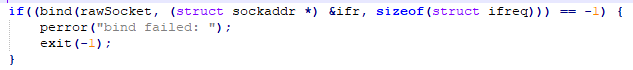
\includegraphics[width=0.9\textwidth]{Bind.PNG}
    \caption{Binding our socket to the interface we want to listen on. }
    \label{fig: Raw Socket Traversal}
\end{figure}

We can now code an infinite loop in C that will allow us to receive sniffed raw packets that have travelled past our raw socket bound interface. This infinite loop will also be the basic loop in our proxy that receives packets from incoming sockets and decides on what action to take with them. To do this, we need to use the {\tt recv()} call which receives messages from sockets and store it into a buffer. The {\tt recv()} takes 4 parameters as such; \\
{\tt \textcolor{red}{ssize\textunderscore t\ recv}\textcolor{blue}{(int sockfd, void *buf, size\textunderscore t len, int flags};}\\


\begin{figure}[h!]
    \centering
    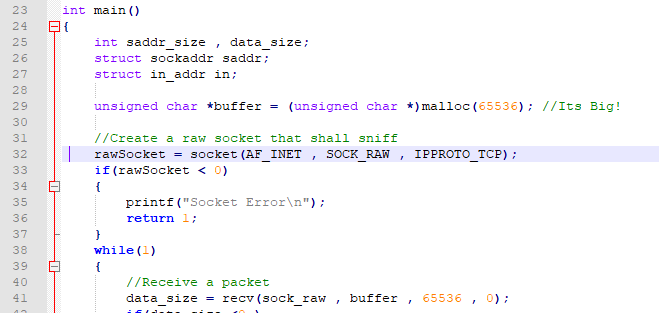
\includegraphics[width=0.9\textwidth]{InfiniteSniff.PNG}
    \caption{Infinite while loop and recv() to sniff packets}
    \label{fig: Recv} 
\end{figure}
                 
From Fig: 4.8, {\tt recv()} is reading from the raw socket we have aptly named {\tt rawSocket} which we have bound to the desired interface previously. Note that the int socket is a file handle as catalogued by the kernel. We have, at this stage, already configured the socket with all the necessary functionality for packet sniffing on an interface. The second parameter is a void pointer to a variable aptly named {\tt buffer} where we will store the incoming packet. The third parameter is the maximum size of this buffer, for which we have allocated memory from the heap via {\tt malloc()}. We use {\tt memset()} to clear the buffer memory to 0, so we have a fresh, clean slate to copy our packets to ~\cite{39}. \\


{\tt \textcolor{red}{// Set up sniffer for incoming packet}\\     
   \textcolor{blue}{unsigned char *buffer = (unsigned char *)} \textbf{malloc}\textcolor{blue}{(65536);} \\
   \textcolor{blue}{memset} \textbf{(buffer, 0, 65536)};} \\
   
The {\tt int flags} (parameter 4) is set to 0.  This sets us up for the next section where we forward packets and begin to send spoofed packets. 

\subsection{Forwarding packets}
Note that for this thesis, we are primarily concerned with the capture and duplication of TCP connection-oriented packets. Once we have established that our sniffer has bound to the desired interface and receives packets, we can start forwarding packets. The task to perform now is to ensure that we can take in an IP packet from our sniffer bound interface and forward it out on another outgoing interface with a new Ethernet header to its destination ~\cite{35}~\cite{38}. A breakdown of the steps is follows:\\

\begin{enumerate}
\item Extract the relevant information from the packet, including header information (source IP address, flags set, checksum) and the data payload. \\
\item Using a library of header structs for IP, TCP  headers to store all the information gleaned from the sniffed raw packets. \\
\item Create new Ethernet packet and forward with a copy of the original packet in it to the intended destination. We do this by allocating memory from a new buffer and utilise the header structs to set the correct fields in the correct places in the buffer. Then pass completed buffer to raw sockets {\tt send()} function.\\
\item Send ACK back to the source to acknowledge reception of the packet with the modified sequence number. \\
\end{enumerate}

We have already briefly explained how the {\tt struct ifreq} was used to extract information from an interface to be used in our raw socket binding. The concept here is the same for step 1 and step 2 where we extract header information. Step 3 also involves another substep of determining the next hop MAC address ~\cite{40}. Unfortunately, in C there is no direct programmatic in-process access to the kernel ARP table. So we have two choices at this point. We could either:\\

\begin{itemize}
\item query the kernel ARP table by starting an additional process which is restrictive if we are trying to process hundreds of packets per second. 
\item build our own ARP table and send our own ARP requests and read ARP replies that are received back.\\
\end{itemize}

We choose the second option. This involves creating our own ARP table cache, creating and sending an ARP request and waiting for the corresponding ARP reply containing the next hop MAC address needed before we can forward a packet. Any data packets (not an ARP reply or response) received will have a source MAC, source IP, destination MAC and destination IP. The destination MAC will be our incoming interface MAC address. The source MAC will be the last hop MAC just before our incoming interface MAC address in the forwarding chain ~\cite{1}~\cite{2}. To forward the packet onwards via our outgoing interface, we must fill in the destination MAC ourselves by either querying our cache table for a MAC entry for the packet's destination IP address or by using the ARP request. We will delve into that in more detail later in Section 4.2.5 "Finding the MAC address for forwarding packets". \\

In the context of forwarding, we could have also used the standard Linux packet forwarding/routing mechanisms. For this thesis, we will construct our own forwarding mechanism with C code ~\cite{39}. The advantages of building our own here is that we get: \\

\begin{itemize}
\item Access to the headers which allows us to eventually rewrite fields such as, for example, the advertised windows.
\item It allows us to decide which packets to forward and which ones we do not want to forward. 
\item It allows us to inject our own packets which we did not receive but have created ourselves (e.g. ACKs)
\item It allows us to cache packets we have forwarded until we receive ACK back from the destination \\
\end{itemize}

As is the standard with any PEP, we will receive the raw packets complete with headers. AS a consideration for future work, We will eventually be able to change the header contents and size of the advertised window to control the flow of traffic so that if there is congestion, we can limit the number of packets sent. If the link is not at capacity, we can make the window bigger to allow more packets through. We will elaborate on this further in Section 4.3 "Our Proposed Solution". \\

\subsubsection{Receiving raw network packets:}
So once the steps of opening a raw socket and binding it to a particular interface for the purposes of capturing/sniffing network traffic have been completed ~\cite{38}, the next step is to save our incoming traffic to our buffer via {\tt recv()}. Saving the packets to our buffer allows us to examine the content of the datagrams/packets (e.g. Ethernet, IP, TCP headers and payload) for our PEP purposes ~\cite{35}. \\

We use the \textbf{\tt recv} API call here that is used to receive entire Ethernet packets messages from the raw socket and store it in our buffer ~\cite{35}. In short, the {\tt recv} call takes the raw socket, the buffer pointer, buffer size and int flag as parameters and returns the length of the message/packet in bytes upon completion. The packet is stored in the buffer, and we can now use this to inspect the packet and extract the various headers (e.g. Ethernet, IP, TCP). This is a crucial step in progressing towards the forwarding of packets in our next section ~\cite{35}~\cite{38}.\\

\noindent {\tt \textbf{\textcolor{red}{//Receive a network packet and copy in to buffer}}\\
\textbf{\textcolor{blue}{bufferLengthInBytes} = recv\textcolor{blue}{(rawSocket, buffer, 65536, 0);}}}\\

The following three subsections, (EtherNet Header Struct, IP Header Struct and TCP Header Struct) assist in steps 1 and steps 2 from the list mentioned earlier at the beginning of this section 4.2.4. The three sections will detail the information extracted from the received raw packets and the structs used to store this information. For example, we need to retrieve a source address to create an ACK, or we need to extract a destination address to forward or send an ARP request. 

\subsubsection*{Ethernet header struct:}
The Ethernet header struct, like all structs in general, can be likened to a class as seen in Java or other high-level object oriented languages. It only has attributes, however, and no methods (See Appendix A).  \\ 

\noindent {\tt Example: \\
{\#}\textcolor{orange}{include}<netinet/ip.h> \textcolor{red}{{\//*} \emph{Provides declaration for IP header}{\/*/}} \\
 {\#}\textcolor{orange}{include}<netinet/tcp.h> \textcolor{red}{{\//*} \emph{Provides declaration for TCP header}{\/*/}} \\
 {\#}\textcolor{orange}{include}</net/ethernet.h> \textcolor{red}{{\//*} \emph{Provides declaration for Ethernet header}{\/*/}}\\
 {\#}\textcolor{orange}{include}<netinet/udp.h> \textcolor{red}{{\//*} \emph{Provides declaration for UDP header}{\/*/}} \\
 {\#}\textcolor{orange}{include}<netinet/ip\textunderscore icmp.h> \textcolor{red}{{\//*} \emph{Provides declaration for ICMP header}{\/*/}} \\
 {\#}\textcolor{orange}{include}</net/if.h> \textcolor{red}{{\//*} \emph{struct ifreq}{\/*/}}}\\

The Ethernet header contains the source and destination MAC address of the received raw packets as well as the protocol of the packets. All of this information can be extracted via an Ethernet header struct from the received sniffed raw packets in our buffer. The source MAC gives us the physical address of the last hop from which the packet came. The destination MAC address is the physical address of the interface we are sniffing. These two MAC addresses are not the addresses we need for the forward leg. To forward the packet, we need to use the packets destination IP address to find the next hop MAC address on the outgoing interface ~\cite{35}~\cite{38}.\\


\begin{lstlisting}
struct ethhdr {
    unsigned char h_dest[ETH_ALEN]; /* destination ethaddr*/
    unsigned char h_source[ETH_ALEN]; /* source etheraddr*/
    uint h_proto; /* packet type ID field*/
}; attributes_((packed));
\end{lstlisting}

Note that the Ethernet header is the first data item in the buffer. Thus the start address of the Ethernet header is the same as the start address of the buffer in memory ~\cite{1}. The struct in its memory layout maps directly on to the raw packet stored in the buffer. Therefore we can use the struct to get access to these fields in our buffer as shown below. Hence, the reason we can cast the buffer with a struct ethhdr pointer and access the all the packet fields ~\cite{38}.\\

\noindent{\tt \textbf{\textcolor{red}{struct} ethhdr *ethhdr} = (struct ethhdr *)(buffer);\\
\textbf{printf(}\textcolor{green}{"destination eth addr is \%02x:\%02x:\%02x:\%02x\%02x\%02x"},
ethhdr->h\textunderscore dest[0], ethhdr->h\textunderscore dest[1], ethhdr->h\textunderscore dest[2], ethhdr->h\textunderscore dest[3], ethhdr->h\textunderscore dest[4], ethhdr->h\textunderscore dest[5]\textbf{)};\\
\textbf{printf(}\textcolor{green}{"source eth addr is \%02x:\%02x:\%02x:\%02x\%02x\%02x"},
ethhdr->h\textunderscore source[0], ethhdr->h\textunderscore source[1], ethhdr->h\textunderscore source[2], ethhdr->h\textunderscore source[3], ethhdr->h\textunderscore source[4], ethhdr->h\textunderscore source[5]\textbf{)};\\
\textbf{printf(}\textcolor{green}{"Protocol is \%lu"}, ethhdr->h\textunderscore proto\textbf{);}}\\

The Ethernet header is typically 14 bytes long. It consists of:

\begin{itemize}
\item 6 bytes for destination MAC address (the physical address the packet is destined for).
\item 6 bytes for source MAC address (the physical address of the last hop the packet came from)
\item 2 bytes for the protocol of the packet. This gives information about the next layer of the packet, e.g., If we get 0x800, then the next header in the buffer after the Ethernet header is an IP header. \\
\end{itemize}

In short, we create a pointer of a type struct ethhdr that points to the start of the buffer. The struct maps the fields in the packet we have in our buffer which allows us to access the packets 6-byte destination and source MAC address and the protocol field. 

\subsubsection*{IP Header struct:}
The iphdr struct is used in the same way as the {\tt struct ethhdr} except, in this case, we have a few more fields to access, and we must move our pointer to the correct position in the buffer, where our IP header begins. \\
{\tt{\#}\textcolor{orange}{include}<netinet/ip.h> \textcolor{blue}{{\//*} \emph{Provides declaration for IP header}{\/*/}} \\

\noindent \textcolor{red}{struct} iphdr *ip = (struct iphdr*) (buffer + sizeof(struct ethhdr));}\\

As seen in the line of code above, our pointer is no longer at the start of the buffer. We increment the pointer by the size of the Ethernet header (14 bytes) so that it points at the beginning of the IP header. The {\tt struct iphdr} above has all the attributes needed to store the information that we will extract from the retrieved raw packets. (See Appendix A to view structure of IP header). As shown in Figure 4.9, shows the IP header fields and these are mapped by the struct iphdr. We can access this information similarly as we did with the Ethernet header struct prior. \\


\begin{figure}[h!]
    \centering
    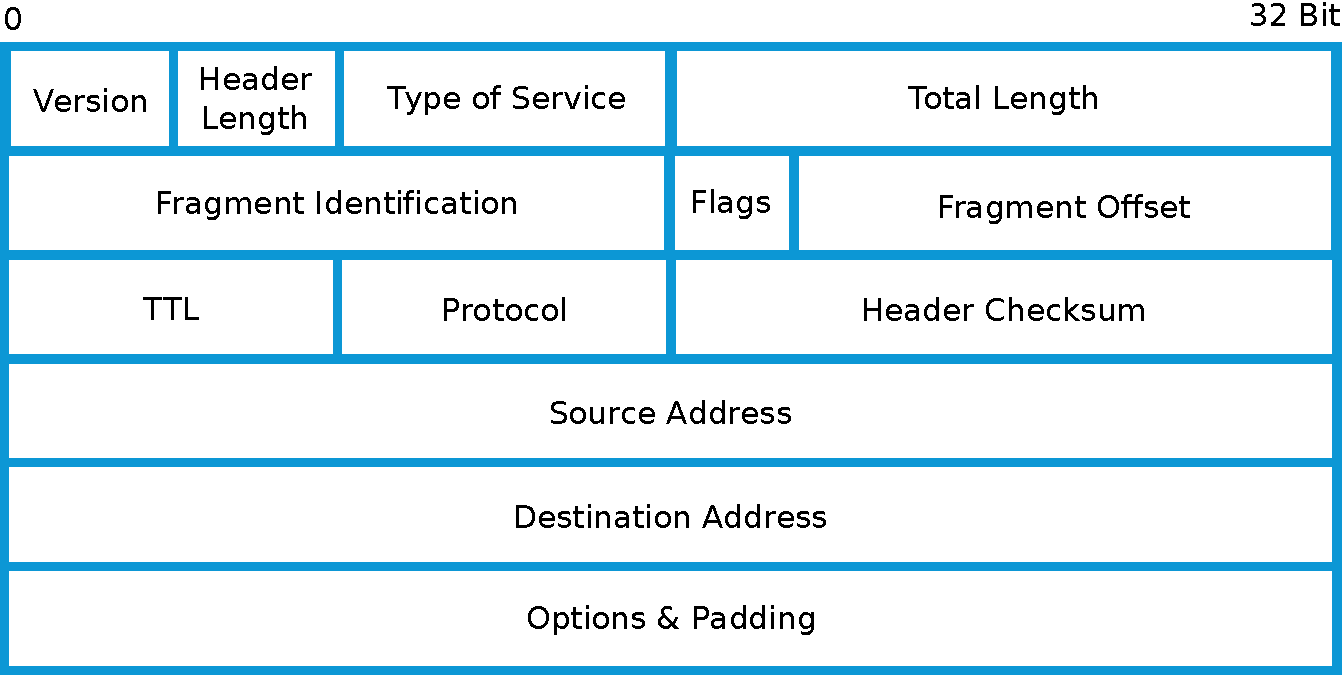
\includegraphics[width=0.87\textwidth]{ipheader.pdf}
    \caption{IP header}
    \label{IPheader} 
\end{figure}

The main conceptual takeaway here is that we are now able to access every field shown in Figure 4.9 of the IP header via the struct ~\cite{35}~\cite{38}. The protocol field, for instance, will tell us whether the upper layer protocol of the packet is UDP or TCP. (If the packet is UDP, our PEP will take no action with it and forward it on. Our PEP only deals with connection oriented protocols). We can calculate the total length of the IP header in bytes, as shown below, by taking the value of the length field and multiplying it by four. The IP header specifies the length of the header in D-WORDS which are 4 bytes in length ~\cite{2}. This knowledge will then allow us to locate the start of any TCP header following the IP header.\\

\begin{lstlisting}
unsigned short iphdrlen;
iphdrlen = ip->ihl*4;
\end{lstlisting}

The main fields we should be aware of are the last two fields, namely source address {\tt (saddr)} and destination address {\tt (daddr)} which are both 4 byte or 32-bit fields in the header and the iphdr struct respectively. The destination IP address {\tt (daddr)} is especially crucial as the {\tt daddr} is needed for the assembly of an ARP request (ARP resolution) which is crucial for acquiring the target destination MAC address that our packet injector will be sending spoofed packets to. The IP header and IP destination address are needed for the end to end connectivity in the network ~\cite{1}. As programmers, we can determine whether we need to manage this packet based on this information. For instance, if the packet is headed to the target network, we need to manage the packet. Otherwise if it is a packet to the local network or alternatively a packet headed specifically to the proxy machine hosting our PEP, we simply forward the packet.  \\

\subsubsection*{TCP header struct:}

Our PEP will deal exclusively with connection orientated protocols, (as do most PEPs generally), so we will focus on Transmission Control Protocol(TCP) rather than UDP. Regarding coding, this means our PEP will read the protocol portion of the IP header in our buffer, and only interact with TCP packets. Non-TCP packets will simply be forwarded without further ado.\\

The TCP header structure as defined in tcp.h can be viewed in Appendix A. It is possible to construct our own TCP struct theoretically, but the TCP header struct already exists in a library which we can easily import. \\

\noindent\textbf{Example of tcphdr struct library import:}\\
{\#}\textcolor{orange}{include}<netinet/tcp.h> \textcolor{red}{{\//*} \emph{Provides declaration for tcp header}{\/*/}} \\

As with the Ethernet header and IP header structs, the concept behind the TCP header struct is precisely the same. The tcphdr fields, as seen in Fig 4.10, will all be accessible via the tcphdr struct (See Appendix A to view the {\tt struct tcphdr} as defined in the tcp.h library). All that is required now is to create a pointer of type {\tt struct tcphdr}. Using our buffer as a starting point, we increment our pointer by the size of the Ethernet header(14 bytes) plus the size of our IP header, so that it points at the start of the TCP header ~\cite{38}.\\

\noindent \textcolor{red}{struct} tcphdr *tcp=(struct tcphdr*)(buffer + iphdrlen + sizeof(struct ethhdr)); \\

Now that we have a pointer to the TCP header in our buffer, we can do the following:\\

\begin{enumerate}
\item We can identify what flags are set which will identify what type of packet we have in our buffer (is it a SYN, ACK, SYN + ACK, FIN, RST?).
\item Being able to identify the type of packet we have will allow us to make decisions about what action we take with the packet. (e.g. do we need to forward it, absorb it, forward it, cache and forward etc.).
\item We can trace the sequence and acknowledgement numbers of the packets. This information will be useful once we begin our proxy functions for our PEP.\\
\end{enumerate}

\begin{figure}[h!]
    \centering
    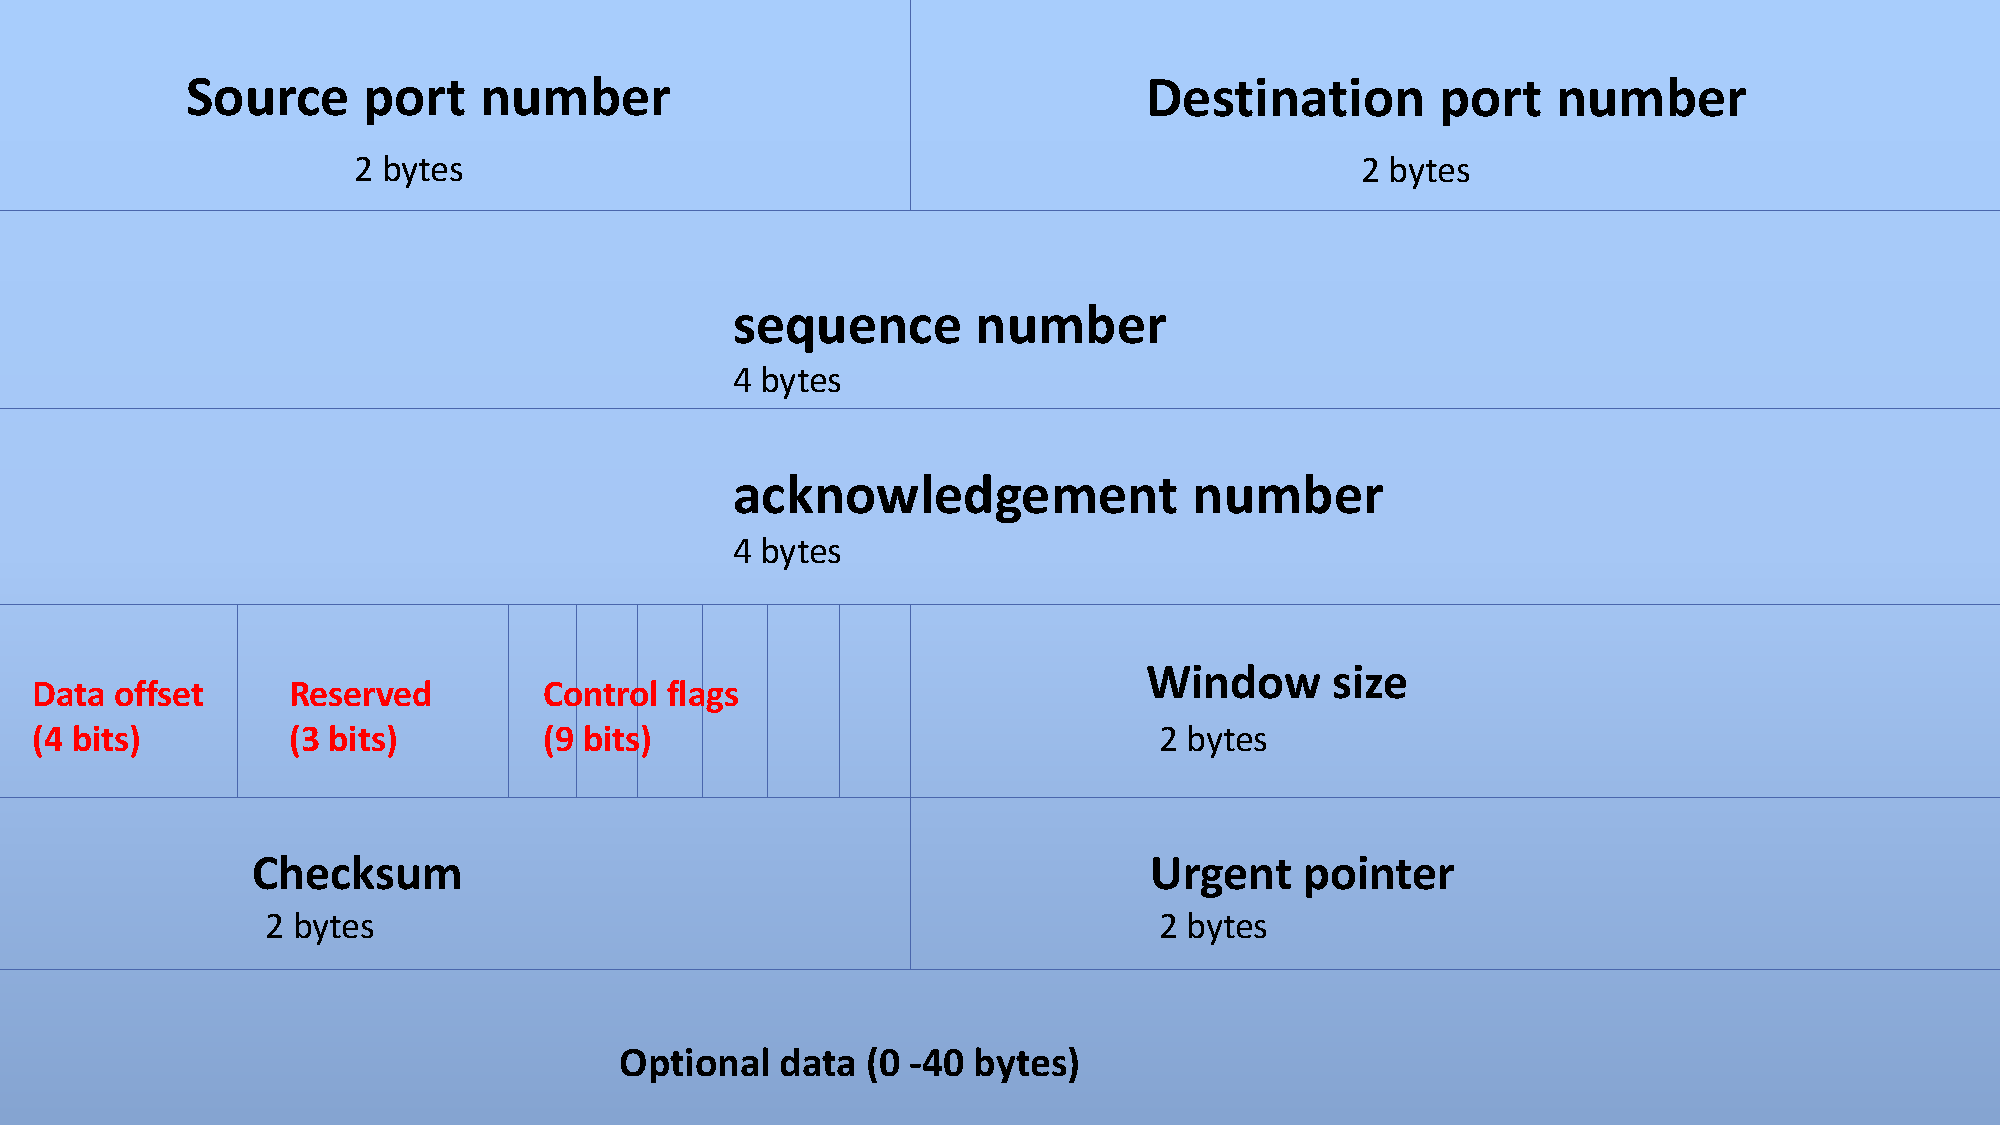
\includegraphics[width=0.95\textwidth]{TCPHeaders.pdf}
    \caption{TCP header fields}
    \label{TCPHeader}     
\end{figure}

These are just a few examples of what can be done. As well as being able to inspect the packets in our buffer, we will also be able to create duplicate packets and alter fields within them to suit our proxy purposes. \\

The control flags are defined in the hexadecimal format each represented by the FIN, SYN, RST, PUSH, ACK and URG flag as number 1, 2, 4, 8, 16,  and 32 respectively. The flags play a key role in our PEP as we will be setting these flags to suit the purposes of our packet injector when we assemble our spoofed packets. When we create an ACK response to a received data packet in our buffer, for instance, we would set the ACK flag to 1 and set all other flags to 0. We would have to create a duplicate of the packet headers but alter the flags so that only the ACK flag is set to indicate this is an ACK response ~\cite{35}. \\

The ACK packet we created would also need to have its sequence number and ACK number set accordingly. The source port number and destination port number fields would also need to be swapped when we create the ACK packet. We would also need to swap the source IP and destination IP addresses in the IP header of the packet. Similarly we must also swap the source and destination MAC addresses in the packets Ethernet header. In all of these cases, this requires the recomputation of the header checksums ~\cite{38}.\\

\subsubsection{Summation of the header structs usefulness for a PEP}
From a conceptual standpoint, the underlying message the reader may wish to take away from these last three sections is that the structs give a programmer the means to do two significant things. Firstly, the structs allow us to read the contents of a packet received on an interface we have bound our raw socket sniffer to. Secondly, the structs allow us to use information from the packets to build our own datagrams and packets for forwarding through our PEP via packet injection. For example, if we receive a raw network packet into our buffer that is a data packet, we can read its source MAC address and source IP address from the Ethernet and IP headers respectively, then replicate them as our destination MAC and destination IP addresses when we construct our ACK packet ~\cite{35}~\cite{38}. We will explore this more in our Proxy chapter. If the received raw packet needs forwarding, we can use the destination IP address to do an ARP lookup in our ARP table cache or to build an ARP-Request Packet. This leads us to our next section on Address Resolution Protocol (ARP) needed for forwarding of packets. \\

\subsection{Finding the MAC address for forwarding packets}
We now have the means to receive raw packets and read the header and data information coming from any particular interface we have bound our raw socket to. We can assemble an ACK reply to send back to the sender based on this information (we can glean their IP and MAC addresses via the sniffer) but forwarding the packet onto its next hop MAC destination requires another step. \\

As Fig. 4.9 shows, the incoming packet will have its source IP address and the destination IP address while the incoming Ethernet header holds its source mac and the destination MAC address (the MAC address of our sniffing interface). Forwarding the message onto the next hop in the Ethernet data link layer requires a destination MAC address, but we only have the destination IP address to help us forward the packet ~\cite{1}~\cite{2}.\\

Usually, the kernel would take care of finding the next hop MAC address for our packet using its own internal ARP table, forwarding the packet out the interface we specified in our C code onto the next hop MAC. This was not the case, however, and the kernel was overriding that command and sending it out the interface it deemed best. Often, the combination of being sent out the wrong interface and the MAC address of the next hop based on that interface, caused many unforeseen problems with our PEP. For starters, it meant that we could not control where the outgoing packets from our PEP would go and that defeats the purpose of having a PEP in the first place. It became clear at this point that we must code for the Ethernet layer and manually set our destination MAC address as well. We needed to create our own Address Resolution Protocol (ARP) request frames and ARP table cache to store these MAC addresses. \\

Address Resolution Protocol (ARP) is the mapping of a layer 3 network address to a layer 2 link layer address in the OSI model. In other words, ARP is used to map an IP address to a MAC address and (vice versa as well) ~\cite{1}. Given we can glean the destination IP address from the sniffed raw packet, acquiring the destination MAC address is achievable in two ways. We can use the destination IP address to look up the MAC in the ARP table. If there is no IP to MAC mapping entry found in the table, then we can retrieve the MAC address via an ARP request and listen for an ARP reply. 

\subsubsection{Brief summary of address resolution protocol (ARP)}
When a host is performing an ARP, the destination IP address the host wants to communicate with is known, but the destination MAC address is unknown. The host will broadcast an ARP request packet that will be received by all other hosts in its local network. \\

\begin{figure}[h!]
    \centering
    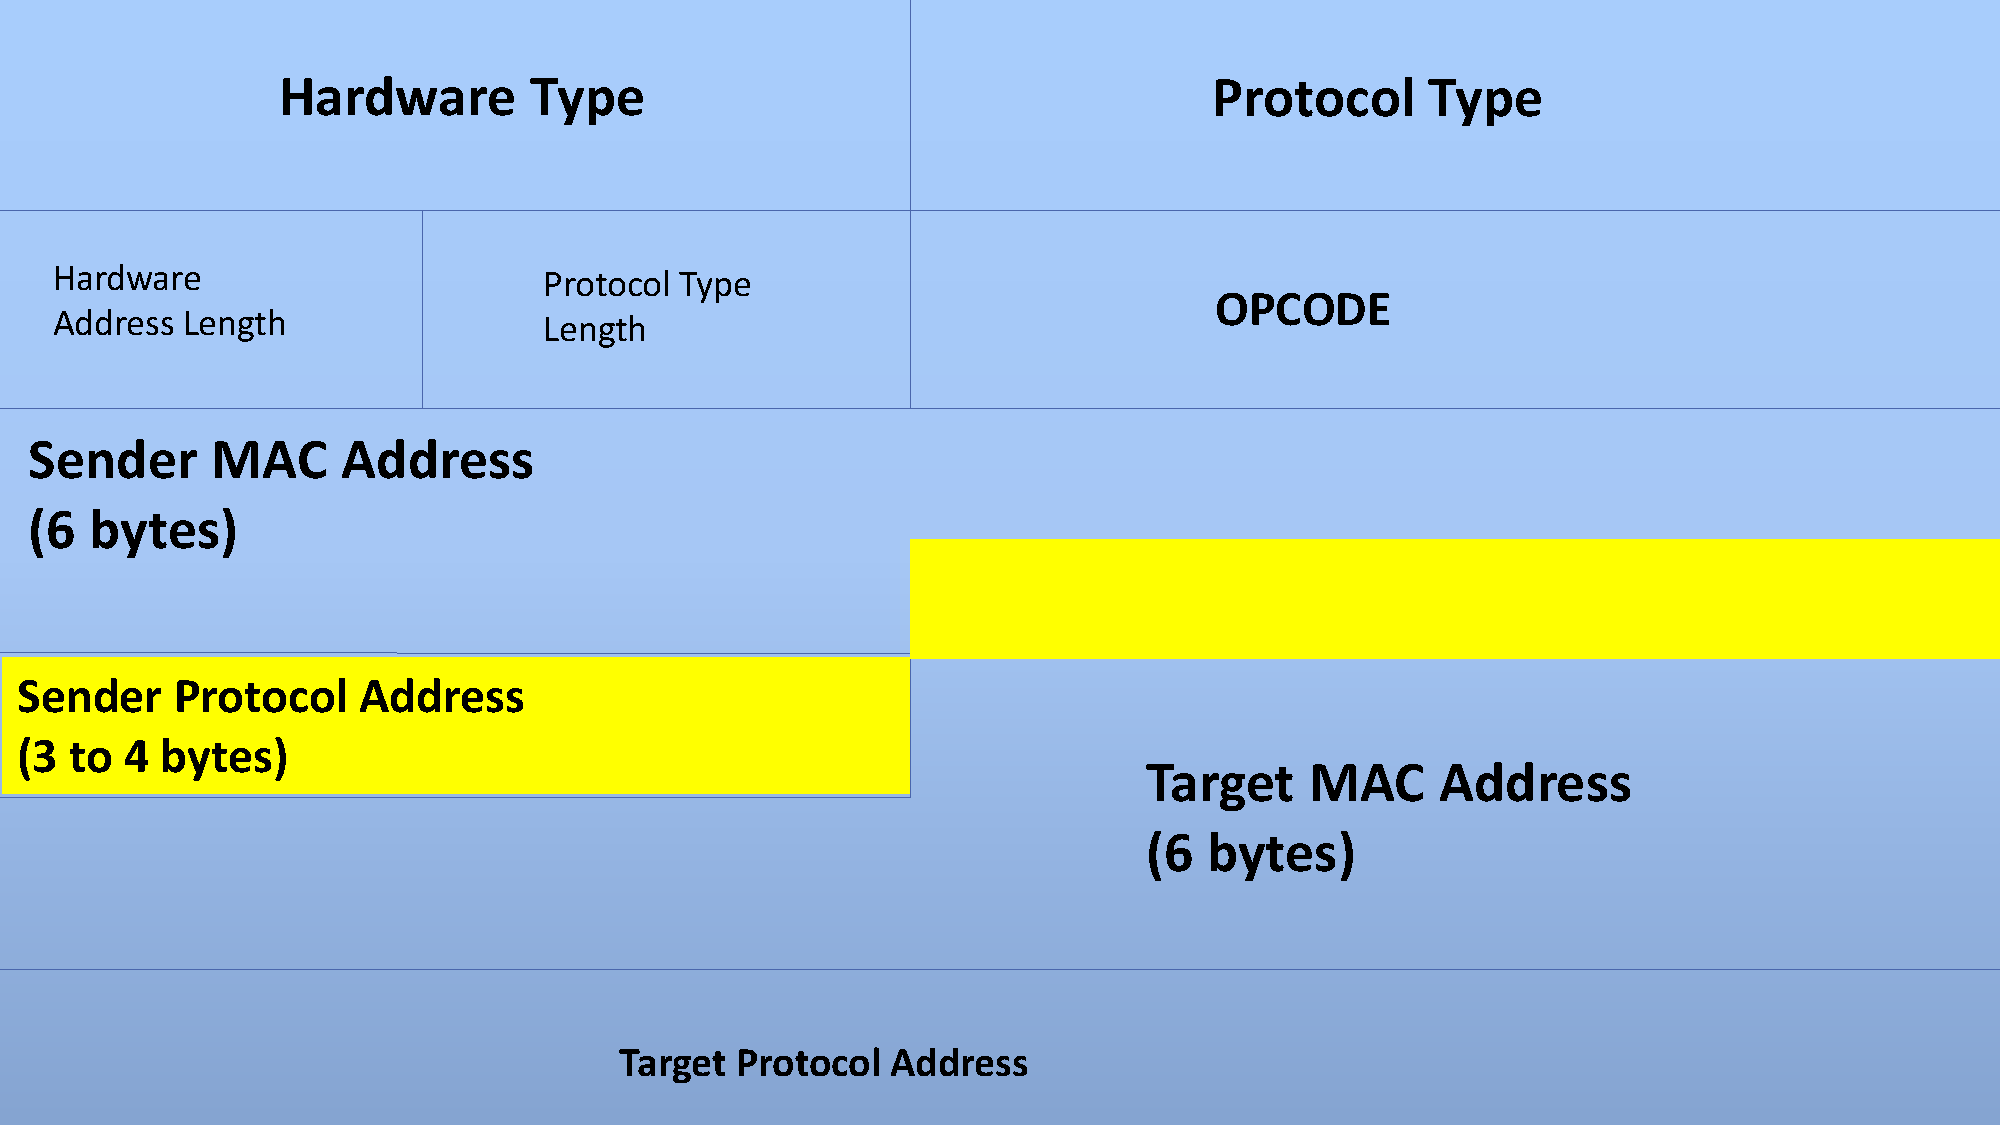
\includegraphics[width=0.95\textwidth]{ArpHeaders.pdf}
    \caption{ARP Header fields}
    \label{ARPHeader}
\end{figure}

It does this by setting the target hardware MAC address field as shown in Fig:4.11 ARP header to all zeroes 00 : 00 : 00 : 00 : 00 : 00. The destination MAC address in the Ethernet header is then set to FF : FF : FF : FF. This is a unique MAC address that ensures the ARP packet is broadcast to every host computer in the local network subnet~\cite{1}~\cite{2}. The concept behind the broadcasting of an ARP request is straightforward. The ARP request is asking each host in the broadcast domain the question "who has this IP address? (destination IP address)". The host computer with this IP address will respond "I have this IP address" and resend confirmation of this with an ARP-Reply packet that is almost identical to the ARP request in structure. The significant difference is that the ARP-Reply will be sent back with the target hosts MAC address as its Sender Hardware Address field ~\cite{1}~\cite{2}. \\

This  Sender Hardware Address is the Destination MAC address information the sender required from the host. The sender can now fill in its packets "Destination MAC address" field in its Ethernet header with the ARP-Reply  Sender Hardware unicast MAC address (singular) rather than the initial broadcast address (FF : FF : FF : FF : FF : FF). The packet is then forwarded to the host on that destination MAC address subnetwork ~\cite{1}. \\

When the destination IP belongs to a network beyond the local network to whom the interface of the current host is connected to  (not an IP on PEPs interfaces subnetwork or local network), the ARP request will retrieve the MAC address of the router interface that is the default gateway to the destination network. The protocols of the routers and switches in the outer network will take care of delivery of the packet from then onwards ~\cite{1}.

If the destination IP belongs to a host in the local network, then the MAC address of that host will be returned to the sender of the ARP request. The next step is to create our own ARP table to track the MAC to IP address mappings. It would not be efficient programming to send an ARP request every time we need to forward a packet. Therefore we need an ARP table which can cache these IP to MAC mappings. The general idea is that our code will check the ARP table first to see if we already have a MAC address mapping for an IP address before sending any ARP-Request packet ~\cite{1}~\cite{2}. (i.e. We initially start with an empty ARP table and we progressively populate the table with the responses to ARP requests that we send. There is also a timeout for each ARP entry).

\subsubsection*{ARP table:}
Each host machine on the subnetwork has an ARP look-up table that keeps a record of the IP address mappings to MAC addresses it finds ~\cite{1}~\cite{41}. Before making an ARP request, the host sender checks its own ARP look-up table to see if it has already ARPed this IP address and thus has the MAC address cached in the table. If so, an ARP request is not required. If there is no existing entry, an ARP request is sent, and upon return of the ARP reply, a new IP address to MAC address record is cached in the ARP table ~\cite{1}~\cite{2}~\cite{41}.\\

\subsubsection*{What We Need To Do:}
This means we need to create an ARP request packet ourselves to wrest control from the kernel. In our case, this also involves creating an ARP struct that will store the ARP reply information when the request is answered and our own ARP look-up table to cache IP address mappings to MAC addresses. As the ARP Header is not readily found in a library for import, we will have to create our own ARP Header struct which is very easily done: \\

Firstly, in dealing with the construction of a basic ARP look-up table, it must be built to allow us to store MAC addresses with their corresponding IP addresses as keys while also having a fast and CPU efficient method of searching for these MAC addresses based on their IP address key ~\cite{1}~\cite{41}. We settled on a binary search tree model for the table that would be able to perform  this function. The first step is creating another struct aptly named "node" ~\cite{42}. \\

\begin{lstlisting}
struct node {
	uint32_t ip;
	uint64_t mac;
	struct node *left, *right;       
}
\end{lstlisting} 

For this thesis, we assume here that the reader is familiar with binary search trees (see Appendix B) ~\cite{42}. There is a function in our code that takes the IP address and our BST node struct ARP table to look up a MAC address in the ARP table. Our code also has an insert function that inserts new nodes to the ARP table. To create our BST search tree ARP table, we simply declare a pointer of type {\tt struct node* arpTable} which we will assign memory to via {\tt malloc()} in a later part of our code ~\cite{39}.

\subsubsection*{ARP header struct}
As in the previous section, our ARP Header struct will contain attributes corresponding to the fields in an actual ARP Header. We are using C language, so we simply declare a variable of:\\

\begin{itemize}
\item \textbf{typedef struct} arpHeader arphdr\\
\end{itemize}

Next we declare our struct that will take on the fields of an actual ARP header:

\begin{lstlisting}
struct arpHeader {
    uint16_t htype;
    uint16_t ptype;
    uint8_t  hlen;
    uint8_t  plen;
    uint16_t opcode;
    uint8_t  sender_mac[6];
    uint8_t  sender_ip[4];
    uint8_t  target_mac[6];
    uint8_t  target_ip[4];
};
\end{lstlisting}

Our C code for our PEP implementation will fill this struct with the information we receive from the sniffer. See Fig 4.12 to see how this is actioned in our C code. \\

\begin{figure}[h!]
    \centering
    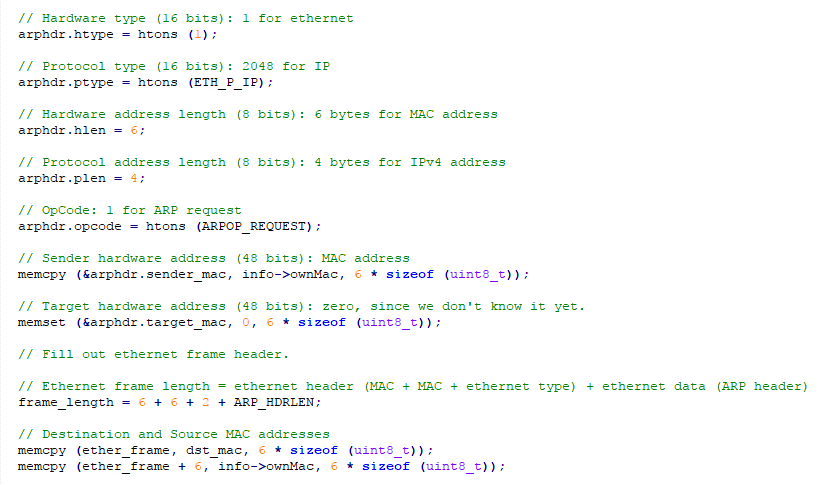
\includegraphics[width=0.9\textwidth]{Capture.PNG}
    \caption{ARP Header}
    \label{fig:Filling fields of ArpHeader struct}
\end{figure}

To summarise, when we receive a packet that needs to be forwarded, we check our ARP table to determine whether we already have a MAC address cached for the destination of the packet IP address. If not, we create an ARP-Request to find the MAC address. Once we have constructed our ARP header, we can send out an ARP request to our local network or the gateway interface.\\

With the destination MAC address returned, we are at a stage where we can now forward the IP/TCP packets we have received on the sniffing interface to their destinations. This leads into the next section which deals with our proposed solution and our methodology for building our proxy logic. \\

\subsubsection{Forwarding the complete packet with the sendto() function}
Once we have a packet assembled and complete with forwarding MAC address, the final step is to forward the packet. Socket programming has a {\tt sendto()} function that completes this process ~\cite{35}~\cite{38}. \\

\noindent{\tt \textbf{bytesSent} =  \textcolor{blue}{sendto}(interface->txSocket, packet->packet, packet->packetSize, 0, (\textcolor{purple}{struct} sockaddr *) \&interface->device, \textcolor{blue}{sizeof} (\textcolor{purple}{struct} sockaddr\textunderscore ll))};\\

The code excerpt above is from the code we use for our PEP. The code makes use of a customised struct created for the incoming and outgoing interfaces of our PEP which will be explained fully in the implementation section of our PEP. The above code also makes use of a struct sockaddr\textunderscore ll (see Appendix B) which allows us to access the link layer for assembly of the Ethernet header. The {\tt sendto()} function takes in six parameters as follows:\\

\begin{itemize}
\item The first parameter is the raw socket we are using for sending: {\tt \textcolor{blue}{int} \emph{sockfd}}.
\item The second parameter is the buffer holding the packet/data for sending: {\tt  \textcolor{blue}{const void} \emph{*buf}}.
\item The third parameter is the length of the buffer: {\tt  \textcolor{blue}{size\textunderscore t} \emph{len}}
\item The fourth parameter are flags which we do not use in our code {\tt  \textcolor{blue}{int} \emph{flags}}.
\item The fifth parameter is the {\tt struct sockaddr} cast pointer to a {\tt struct sockaddr\textunderscore ll} named \emph{device} (see Appendix B) which is a field in the abovementioned customised struct for the incoming and outgoing interfaces of our PEP. The {\tt struct sockaddr\textunderscore ll} contains the forwarding MAC address for the packet/data that is being sent: {\tt  \textcolor{blue}{const struct} sockaddr \emph{*dest\textunderscore addr}}.
\item The last parameter is the size of the struct sockaddr\textunderscore ll in bytes: {\tt  \textcolor{blue}{socklen\textunderscore t} \emph{addrlen}}.\\
\end{itemize}

If the packet is sent successfully, the call returns the number of bytes sent. On error, -1 is returned. This completes the forwarding packets section. The next section covers our proposed solution and the PEP logic and implementation in detail ~\cite{35}~\cite{38}.

\section{Our proposed solution}

As mentioned earlier in the PEP history section, most PEP implementations which deal with satellite link latency adopt the TCP-splitting/connection breaking architecture ~\cite{6}~\cite{14}. Recall that a connection-breaking PEP terminates the connection from one end and opens a connection to the other, such that there are two different connections with different packets, sequence numbers, congestion windows and advertised windows, etc., between the PEP and the two respective endpoints. In a connection-breaking PEP, only the TCP payload data in the packets moves from one connection to the next ~\cite{6}~\cite{14}. The solution offered in this thesis is a non-connection breaking PEP because:\\

\begin{itemize}
\item The PEP does not de-encapsulate TCP packets such that only the payload gets forwarded. The same data packets are seen either side of the PEP, except that retransmissions of packets are only seen on the side of the PEP on which they were lost.
\item The sequence numbers on forwarded packets remain the same. 
\item Only the original TCP sender maintains a congestion window, at least at this point. Future modifications to our PEP may also maintain this window.\\
\end{itemize}

It will, however, interfere with the connection by: \\

\begin{itemize}
\item inserting ACKs when there are none from the receiver yet.
\item intercepting ACKs when an ACK has already been sent to the sender by the PEP.
\item rewriting the TCP checksum and in future/modified versions of this PEP, possibly the advertised window to the sender.\\
\end{itemize}

Our PEP solution aims to partially mitigate some of the problems caused by breaking the end to end rule of the Internet. The next section will elaborate on what these problems are, and then this thesis will outline the proxy functions of our PEP. 

\subsection{Non-Connection breaking PEP}
The novelty of our solution is that it does not break the end to end architecture of the Internet which in turn breaks end to end reliability at the transport layer ~\cite{6}~\cite{13}~\cite{14}. \\

Breaking the fundamental end to end principle of the Internet can create issues in itself. Connection breaking PEPs will not be able to deal with IPsec connection flows or Virtual Private Networks. Encrypted packets under an IPsec flow, for example, will encrypt the IP Payload which includes the TCP header. Connection breaking PEPs need to be able to read the TCP header of the packet in order to send ACKs back to senders and to perform the optimisation procedures effectively. IPsec prevents the reading of TCP headers and therefore hampers these connection breaking PEPs ~\cite{14}.\\ 

Another issue that may arise from the breaking of the end to end TCP semantics is the "Where's the money" problem that results from the consequent breakage of TCP end to end reliability ~\cite{13}. This is one \textbf{real world} negative consequence of violating the end to end TCP semantics of the Internet whereby we have an intermediate agent sending ACKs back to a sender rather than the actual final receiver. Imagine a scenario where one is doing an Internet transfer of money over a connection breaking PEP link satellite connection. \\

TCP client sends the transfer over the line and the intermediate agent PEP, acting as a proxy server, sends an acknowledgement back to the client confirming the transmission of said funds before creating and forwarding the transfer information to the final receiver. These actions break the fundamental end to end connectivity principle of the Internet but will cause no issues so long as there are no problems in the connection. \\

Problems can arise, however, if there is some break in the connection between the PEP and the final receiver before getting the actual information to the final receiver end. In this case, we are left with an undesirable situation where the sender has received an ACK from our intermediate agent PEP but the data forwarded on by the PEP is lost before it reaches the final receiver ~\cite{13}~\cite{14}. Thus the client believes it has transferred the money successfully when the request for transfer of money to the Internet banking site has actually been lost. This thesis puts forth a non-connection breaking PEP that is an alternative to current end to end breaking PEPs. \\

Unfortunately, our non-connection breaking PEP also does not completely solve this problem yet. The PEP preserves port numbers and sequence numbers and is therefore compatible with protocols that include references to these in TCP payloads (VPNs in particular). The PEP also addresses the breaking of the IPsec flows as our proxy would simply forward these packets without ACKing them to the sender. Our PEP, however, does not optimise IPsec flow performance over the link either. The next section will walk the reader through the proxy logic for our PEP in this thesis.

\subsection{PEP proxying roadmap}
Thus far, this thesis has covered the concept of sockets, raw sockets to create a sniffer and the various data structures used to store packet information gleaned from a sniffing (i.e., bound to our raw socket) interface. The forwarding and assembling of packets via these structs have also been covered. This section of the thesis moves now into the most important phase of our PEP construction: The proxy logic.\\

In other words, this part of the thesis takes the reader through the actions and decisions our PEP will make as datagrams/packets traverse through the PEP. The next section will give more detail on the actual implementation of the PEP, as well as outline the PEP logic that we managed to implement (some aspects of PEP logic had to be left to future work due to time constraints). The results chapter will document the performance of our PEP on our lab's Pacific Islands satellite network simulator.\\

Our PEP will be dealing with multiple TCP connections at any one time. To keep track of these connections, our PEP will need a connection table similar to the ARP table used to keep track of IP to MAC mappings. For this purpose, we will once again use a binary search tree structure. Each node will represent a TCP connection, and within each node, we have a FIFO (first in first out) linked list data structure to represent the data packets from each TCP connection that we cache ~\cite{43}. More detail on the implementation of these structures for our connection table will be given in the next section. \\

This thesis assumes that data structures such as FIFO queues implemented as linked lists ~\cite{43}, are known to the reader. The PEP logic works as follows: \\

\noindent \textbf{Filtering the packets; choosing which packets to proxy} \\
Suppose we have now set up the PEP and it is active and ready for operation. The first action our PEP takes upon receiving an incoming packet is to decide whether it is a packet we need to handle. Our PEP code has a function called {\tt checkRXInterface()} which executes this vetting action of us. This {\tt checkRXInterface()} function will look at all the packets being received on the PEPs incoming interface and simply filter out the packets the PEP should ignore, and enqueue the rest of the packets on the interface's receive queue ({\tt rxQueue}) for processing. \\ 

\emph{For our PEPs incoming and outgoing interfaces, we created a struct called {\tt proxyInterface} that has a receive queue for processing incoming packets and a transmit queue ({\tt txtQueue}) for processing transmission of packets.  More detail will be given in the proxy logic implementation section.} \\
 \begin{figure}[h!]
    \centering
    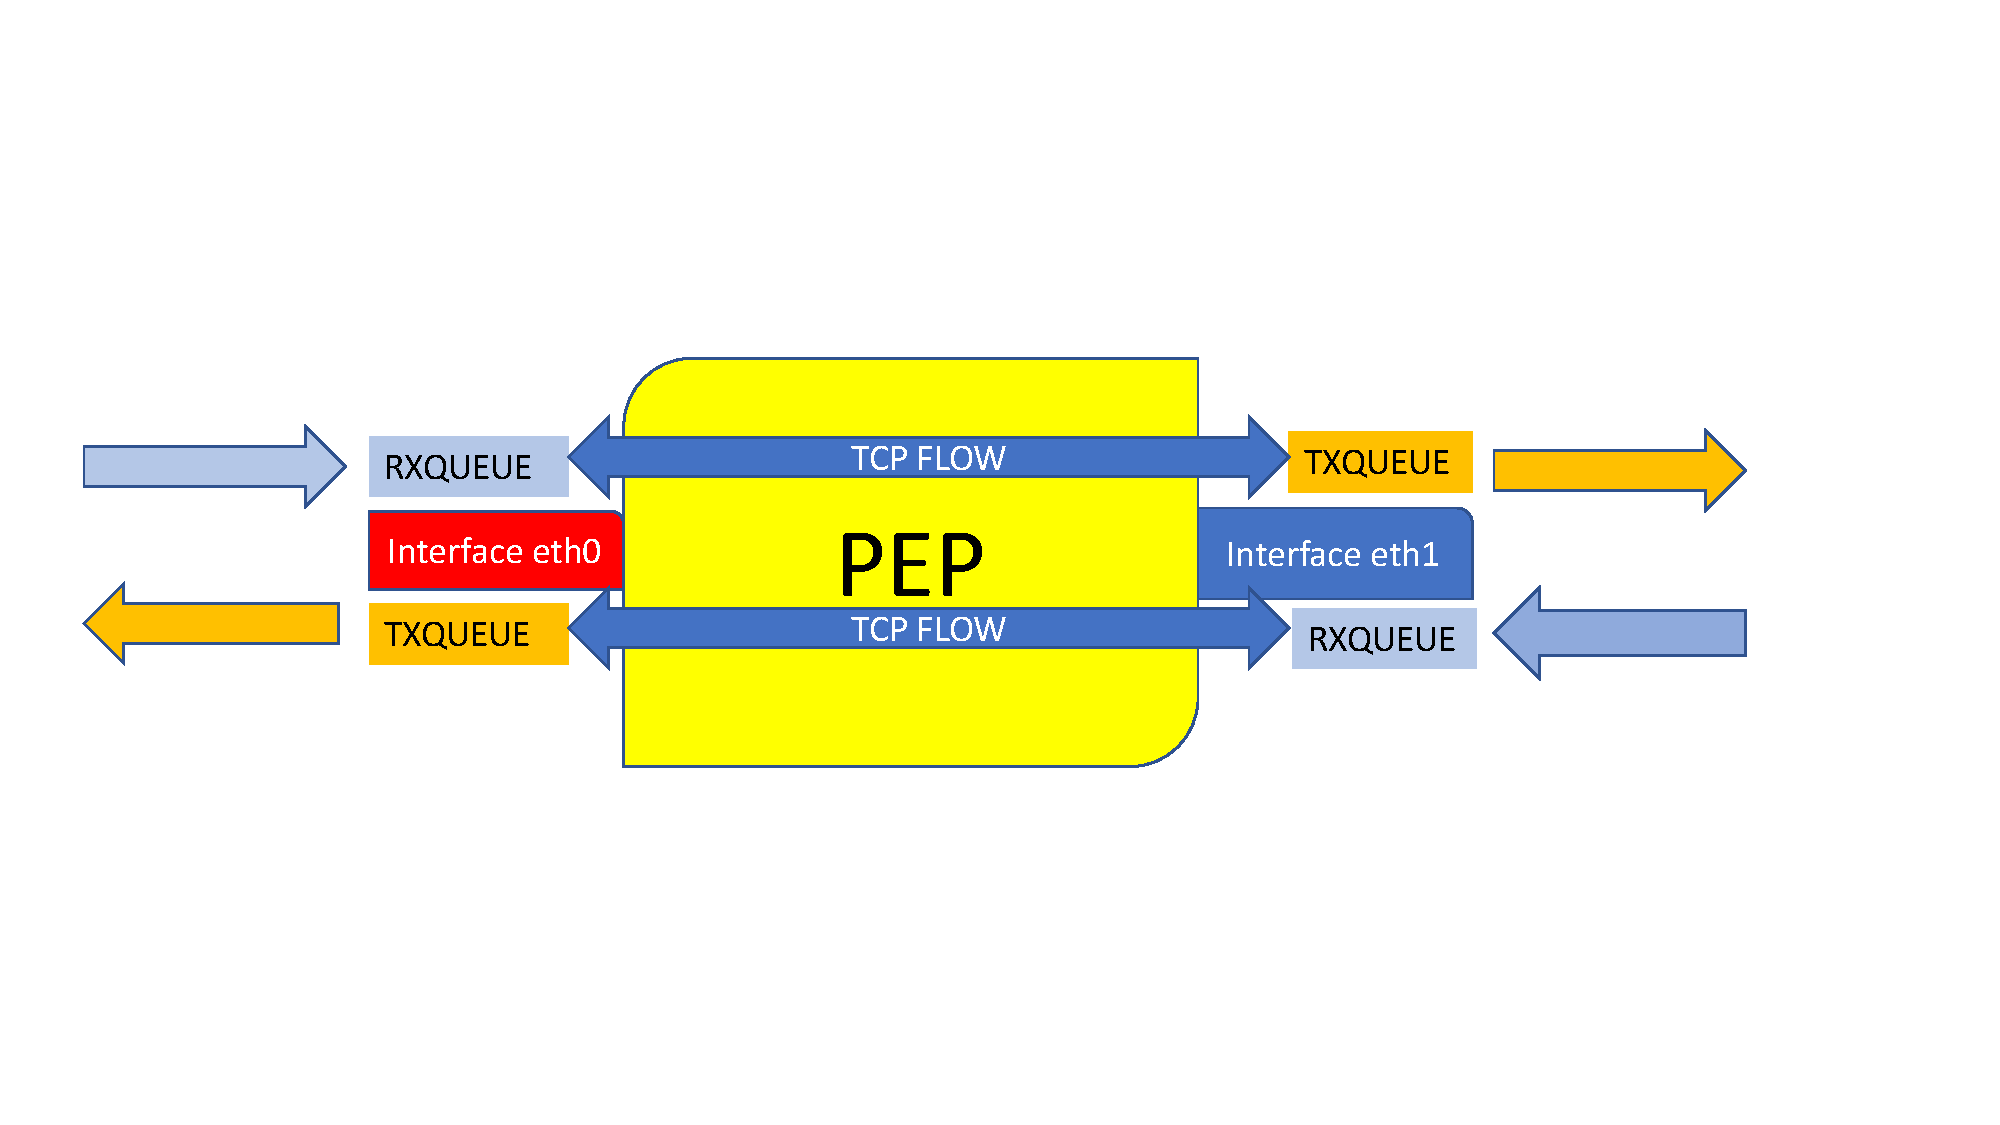
\includegraphics[width=1.0\textwidth]{PEPInterfaces.pdf}
    \caption{The rxInterface and txInterface FIFO queues for both the islandside (eth0) and worldside (eth1) interfaces of the PEP. Note that rxQueues => queueing incoming TCP flows and txQueues => queueing outgoung TCP flows on our PEPs proxyInterface struct.\\}
    \label{PEPInterfaces}
\end{figure}

\noindent \textbf{List of incoming packets our PEP will disregard:}\\
 
There are only three types of incoming packets our PEP will ignore:\\
\begin{itemize}
\item The packets that our own PEP has transmitted and detected on the PEPs  own interface.
\item The packet is directed to the proxy host (i.e., someone is sending data to the computer that our PEP is running on). Our PEP does not need to deal with these packets. There will be other processes on the host computer that can deal with this data.
\item It is a packet directed to another host on the local network of the PEP interface. This host sits on the same side of the PEP as the PEP interface that the packet came in from. \\
\end{itemize}

\noindent \textbf{List of packets our PEP will interact with:} \\

There are only two types of incoming packets our PEP will handle:\\
\begin{itemize}
\item Packets that need to be proxied (i.e., packets that are heading to a network on the other side of our PEP).
\item ARP response packets for an ARP request sent from our PEP. \\
\end{itemize}

The packets listed above are the only ones we are concerned about and that our PEP is designed to proxy (Non-TCP packets will be forwarded on, the PEP will ignore all other packets). The PEP will then enqueue these packets, from the list above, on an interface receive queue (rxQueue) where they will identify the packet as per the list below and apply the appropriate proxy logic accordingly:\\

\noindent \textbf{Applying the proxy logic:} \\

\noindent A) When the PEP identifies an incoming TCP data packet, it must:\\ 

\begin{enumerate} 
\item Identify the TCP connection it belongs to by checking our connection table. If no entry for this packet exists, the PEP creates a new entry for it in our connection table. \\
\item Acknowledge the packet to the original sender (which may have been a PEP on the far side of the sat link, or the original sender). The ACK will eventually need to reflect (in its advertised window field) an idea of how "full" the link currently is. The PEP will know this because it can be configured with the link's queue capacity and because it knows how much data it has sent to the link recently (future work). \\
\item Forward the packet to the final recipient (which theoretically may sit behind another PEP). \\
\item Cache the packet (unless it is already in the cache, i.e., we have received retransmission in which case we resend an ACK to sender) in the FIFO queue of the corresponding TCP connection node in our connection table. (We want to keep a copy of the packet in case we need to retransmit it. If we do not receive an ACK back from the final receiver within a certain allotted time, we assume the packet has been lost/dropped and must retransmit).\\
\end{enumerate}

\noindent B) When the PEP identifies an incoming packet that belongs to a TCP IPsec connection or VPN connection:\\

\begin{enumerate}
\item Do not proxy. Treat as an unknown protocol.
\item Forward all packets from this connection flow onto next hop without alteration. (Note, all non-TCP protocol packets are also forwarded in the same way).\\
\end{enumerate}

\noindent C) When the PEP sees an incoming ACK for a data packet it has cached (i.e., already ACKed to the original sender), it must:\\

\begin{enumerate}
\item Identify the TCP connection the ACK belongs to by checking our connection table. 
\item Delete data packets that the ACK relates to from the cache. This includes any packets whose TCP sequence number + TCP payload length is \emph{below} the ACK number in the ACK packet. Do not forward the ACK packet.
\item Dynamically recalculate the RTT. This calculation is based on the time we receive an ACK, minus the time of sending for the packet with the highest sequence number covered by this ACK. (When our proxy sends a packet, it is also cached simultaneously. Thus we can find the precise time we send a packet via its time of insertion into our cache).
\item Relays the time of the \emph{updated RTT} x 1.3 to another function (housekeeping function which will be detailed later) which periodically traverses the cache and uses this time period to schedule retransmission of unACKed packets. Simply put, the function determines which packets have been in the cache for a time of \emph{RTT x 1.3} or longer, and retransmits them.

\item If the ACK does not cover any data packets in the cache, forward the ACK. It is probably either a duplicate ACK or part of a FIN + ACK, for example, and needs to be forwarded on.\\
\end{enumerate}

\noindent D) When the PEP sees an incoming FIN or FIN+ACK packet for a connection, it must:\\

\begin{enumerate}
\item Forward the FIN or FIN+ACK to the recipient.
\item Set an expiry time on any data packet entries in the outgoing interfaces cache for this connection.
\item Remove the connection from our connection table after the previously mentioned expiry time has elapsed. \\
\end{enumerate}

\noindent E) When the PEP sees an incoming RST packet for a connection, it must:\\

\begin{enumerate}
\item Forward the RST to the recipient.
\item Delete any data packet entries in the cache for this connection on incoming and outgoing interfaces.
\item Remove the connection from our connection table. \\
\end{enumerate}

\noindent F) When the PEP sees an incoming ARP packet, it must:\\

\begin{enumerate}
\item Check if it is an ARP request or ARP response. If it is an ARP request, PEP takes no action. Kernel will handle the request.
\item It is an ARP response. Check if the sender IP address contained within the ARP response is already in the ARP table. If not, add new sender IP to MAC entry in the table.
\item Enqueue any packets that were waiting for the MAC address to arrive. \\
\end{enumerate}


\noindent \textbf{Housekeeping for the PEP:}\\
In addition to the reactive PEP logic described above, it is also imperative to maintain regular housekeeping for the PEP [6]. The housekeeping aspect of the PEP periodically performs a set of actions that clean up our PEP packet caches and keep them up to date. These actions include:  \\ 

\begin{enumerate}
\item Regularly traversing the data packet caches of all active TCP connections utilising our PEP. As the housekeeping function traverses the data packet caches, it will retransmit all cached packets within a TCP connection node, which have not been ACKed within 1.3 x the expected round trip time (RTT). \\
\end{enumerate}

\noindent The housekeeping function should also take care of cached packets that belong to terminated connections and also act accordingly for cases where a receiver has become unavailable. Perhaps the receiver has malfunctioned, or there is some network issue preventing it from receiving packets. Whatever the reason, this scenario must be taken into account:  \\ 

\begin{enumerate}
\item If the housekeeping function comes across cached packets whose expiry time (after a FIN or FIN+ACK) has passed, the function will not retransmit these packets. The expired time signals that the TCP connection has terminated by this stage, so any cached packets belonging to the terminated connection need clearing instead.\\
\item It is necessary to set a cap on the number of retransmissions permitted for any packet (which could be made configurable eventually. We currently hardcode this number.). If a maximum number of transmissions is not set, we could get undesirable effects such as the receiver being unreachable for some reason, but our PEP is continuously trying to retransmit the packet ~\cite{6}. To prevent this, we will set a cap such that if the number of retries reach the cap, we stop retransmitting the packet. In a future modification of the PEP, we may send a RST packet to both end hosts.\\
\end{enumerate}

When we first activate our PEP, we must initially configure an RTT timeout value based on an estimate. Bear in mind that this PEP is being designed with the Pacific Island satellite Internet connection scenario in mind ~\cite{3}~\cite{4}. Our PEP will be tested on the University of Auckland's satellite testbed which simulates the satellite connectivity for the Pacific region covering Niue, Tokelau and Rarotonga [21]. Therefore we can base this first RTT timeout estimate on the Pacific island satellite infrastructure. The most commonly used type of satellite link in this region is through geostationary satellites.\\

For example, when the PEP sits on the world side of a GEO sat link to an island, data packets that made it to the island receiver should be acknowledged no later than the satellite RTT (~500 ms) plus whatever the maximum queue sojourn time at the satellite input is (depends on link rate and queue capacity), plus any small delays on router queues and for processing on the island ~\cite{4}. The latter two components will be small - just a few ms (say less than 10). So if we have a 16 Mbps link (2 MBps) with a 1MB queue, the queue sojourn time is ~500 ms, and all ACKs should have arrived after at most 1010 ms. Once the first ACK is received, our ACK function will dynamically calculate a new RTT and subsequent new cache packet timeout for retransmission from this time forth.\\

\subsubsection{PEP flowchart for PEP logic}
This PEP flowchart features one more important element in our overall PEP logic that has not been mentioned as of yet. Thus far, this section has discussed a TCP connection table (binary search tree structure) for keeping track of TCP connections and the caching of packets in FIFO queues (linked list structures) within the TCP connection nodes ~\cite{42}~\cite{43}. We also modified our ARP table nodes to include the FIFO queue field for storing of packets awaiting MAC address from ARP responses for a particular IP address. To recap, the reason these packets are being cached in these FIFO queues is that: \\
\begin{enumerate}

\item The packet has been forwarded, but we are keeping a copy of the packet in cache until we receive an ACK back from the final recipient. If we receive an ACK within the estimated RTT, we remove all cached packets covered by the ACK. If not, we assume the packet has been dropped. The packet will then be retransmitted via the housekeeping function. \\
\item The packets are awaiting a next hop MAC address via an ARP response before they can be forwarded. The ARP table has been checked, and no entry was found, so an ARP Request was sent. If a response is not received within an allotted timeframe, another ARP Request must be sent. \\

\end{enumerate}

\begin{lstlisting}[language=C]
struct {
    uint32_t ip;
    uint64_t mac;
    node *left, *right;
    time_t insertTime;
    packetQueue * packets;
};
\end{lstlisting}

\noindent \textcolor{blue}{The struct node for the ARP table contains a FIFO linked list queue. The \textbf{\textcolor{red}{{\tt packetQueue* packets}}} is a waiting queue for packets that do not have a MAC for forwarding yet}\\


If we have a packet that needs forwarding and we do not have a MAC address for it yet, the packet is placed in the ARP table entry node queue above and will then be enqueued to the interface transmission queue from there once a MAC arrives from an ARP response. In all other cases, the packets are put straight into the interface transmission queue when we have an existing MAC. In future cases, to avoid complication, we will just assume that this is what the PEP does if we do not have a MAC address. Thus for subsequent sections, the thesis will only discuss queueing packets at the transmission interface, but for simplicity, the reader can remember or keep in mind that this means we may have to queue them at the ARP table entry first.\\


At some point, all of these FIFO queued packets need to be handled, sorted and processed accordingly. The missing element that ties all of these processes together and completes our PEP logic is a struct we created for the sniffing interface:\\
\begin{lstlisting}
struct proxyInterface {
    const char * name;
    uint32_t ip;
    uint64_t mac;
    uint32_t netmask;
    uint32_t network;
    uint32_t gateway;
    int rxSocket;
    int txSocket;
    struct sockaddr_ll device;
    struct packetQueue* rxQueue;
    struct packetQueue* txQueue;
    struct node * arpTable;
    struct connectionCacheNode * cache;
    int cacheConnections;
    int cachePackets;
    int arpEntries;
    int arpPackets;
    int retries;
};
\end{lstlisting}

Note that the struct proxyInterface contains two other structs that we have discussed in the previous chapter. We have the connectionCacheNode* cache which is for the binary search tree TCP connection table ~\cite{42}. (Each node in the binary tree represents a separate TCP connection) ~\cite{42}. The struct proxyInterface also has the previously discussed struct node* arpTable for IP to MAC mappings.\\

With the help of the ifreq struct discussed earlier, we will be able to transfer all the necessary fields for the interface we have bound our PEP to. (e.g. interface IP, mac, netmask, network, gateway IP). The main two new features of our customised struct, however, that this section would particularly want to draw the reader's attention to, are the struct packetQueue* rxQueue and struct packetQueue* txQueue because they both relate directly to our PEP logic flowchart. (Also worth a mention is the struct node* arpTable as we have added a struct packetQueue* field within that node struct to store packets that are awaiting a forwarding MAC address from an ARP response).\\

The struct packetQueue is as its name implies it to be: a queue for packets. The reader may recall that this is the same customised linked list struct we have used to create our FIFO queues in our binary tree connection-table cache nodes (See Appendix B).\todo{promise} In this instance, we use these queues for the packet flow on the interface.\\

The rxQueue (receive queue) represents the queue of packets coming into the interface. Most of the PEP logic is associated with this queue as our PEP makes all of its decisions based on the type of packets that are being dequeued off the rxQueue. (See PEP logic in Proxy RoadMap section). For example, if we receive a packet that has no MAC mapping in the arpTable, we resend an ARP request and queue it in the arpTables packetQueue struct where it will remain until it receives an ARP response.\\

The txQueue (transmission queue) is much simpler as it represents the packets ready to be sent out from the interface. For example, this would include the arpTable packet that has just received an ARP response packet. Our code logic will enqueue the packet on the interface txQueue ready for transmission. \todo{add these structs to Appendix} \\

The programming of the PEP  ensures it traverses and processes the rxQueues and txQueues in a continuous loop. In the main function (of our code), we have these process functions set up in a perpetual \emph{while loop} so that we are continually enqueuing packets coming into our interface on the rxQueue and packets forwarded from our interface in the txQueue. The housekeeping function is also repeatedly called in this perpetual loop but an \emph{if statement} surrounds the function with a timer condition to make sure it is only executed at timely intervals (more detail on the timing mechanism will be given when discussing the implementation of the housekeeping function later in the thesis).\\

The flowchart/use case diagram provides a visualisation of the PEP logic and how it interacts with the interface queues. \todo{make flowchart and place here}It may be useful for the reader to refer to this chart when reading through the PEP logic section and it may also be useful for the next section "Implementing The Proxy Logic In Our PEP" which will frequently refer to the PEP logic often. 

\subsection{Implementing the proxy logic in our PEP}
In the previous section, this thesis presented a high-level overview which gives a walk-through of the PEP logic detailing how the PEP reacts to different TCP scenarios.  The thesis divided the PEP logic based on five different scenarios labelled as A, B, C, D, E, F. This section will go through each of these scenarios and explain how we implemented the logic using the previously covered concepts of raw socket programming, packet sniffer/injectors, and various structs.  This section will also discuss why we chose to fashion our PEP logic in this way. \todo{this a promise...remember to ref back to this} \\

\subsubsection{Scenario A: when the PEP identifies an incoming data packet:}
For this scenario, our PEP performs four sets of actions as listed in the previous section. To recap, the PEP first identifies the TCP connection a received packet belongs to by checking the connection table and making a new entry if one does not exist. Remember that there may be multiple TCP connections traversing through the interface our PEP is listening to. Secondly, the PEP creates an ACK and sends this back to the sender to acknowledge the packet. Thirdly, the PEP forwards the packet to the final receiver. Finally, the PEP caches the packet in the FIFO queue field of the TCP connection node.  \\

As stated earlier, we will be using a binary search tree structure as a connection table, and each node on the table will represent a separate TCP connection. With our ARP table binary search tree data structure, we stored IP to MAC address mappings with the IP addresses acting as search keys within the tree. The question here is how we will be mapping a received packet to a TCP connection? What key is to be used to identify whether a packet belongs to a particular TCP connection? The answer is relatively simple. Every TCP connection flow between two hosts in a network can be uniquely identified by four fields in any packet:\\

\textbf{TCP connection key - forward direction} \\

\begin{tabular}{|l|r|}
	\hline
	Source IP Address & 4 bytes\\
	\hline
    Source Port Number & 2 bytes\\
	\hline
    Destination IP Address & 4 bytes\\
	\hline
    Destination Port Number & 2 bytes\\
    \hline 
\end{tabular} \\

For every packet received via our rxQueue, which we will dequeue one by one, a function generates a 12-byte key consisting of these four fields in this order. Note that every other packet in this TCP connection flow coming from a forward direction into the PEP will also show the same key. As shown in the earlier sections, we use the IP header and TCP header structs to extract this information from our dequeued packets. The generated key identifies these packets as belonging to a particular TCP connection flow.
\\

The PEP will enqueue these packets on either the ARP table packet queue to await a MAC address for forwarding or if a MAC address is already available, straight to the outgoing interface txQueue for transmission. (Once the packets in the ARP table queue receive a MAC address via an ARP response, they will also be enqueued onto the outgoing interfaces txQueue). By default, the PEP will cache a copy of each enqueued TCP data packet when it leaves the interface txQueue at the time of transmission. These packets are then stored, in a FIFO queue, within the corresponding TCP connectionCacheNode. The PEP  caches these packets in case the packets are lost en-route to the final receiver and require retransmission (see PEP Roadmap section).\\

Every TCP connection consists of two flows, one flow in each direction ~\cite{1}. The process described above only handles the forward direction. If for a particular TCP connection, the traffic in the forward direction consists mostly of TCP data packets, then the traffic in the opposite direction will comprise mainly of ACKs ~\cite{1}. We need to use these ACKs to remove packets from our cache, that according to the ACK, have arrived at the receiver. Therefore we also need a reverse key consisting of IP addresses + port numbers for this backward direction. This reverse key will identify which TCP connection an incoming ACK packet belongs to so we can clear the FIFO packet cache in the corresponding TCP connection node. \\

\textbf{TCP connection key - backward direction} \\

\begin{tabular}{|l|r|}
	\hline
    Destination IP Address & 4 bytes\\
	\hline
    Destination Port Number & 2 bytes\\
    \hline 
    Source IP Address & 4 bytes\\
	\hline
    Source Port Number & 2 bytes\\
	\hline
\end{tabular} \\

The key has precisely the same fields as the forward key, except we swap the destination IP address and port numbers with the source IP address and port numbers. When we are sending packets back to the sender host as in an ACK, for example, their packets' source IP and source port numbers become our destination source IP and port numbers respectively and vice versa. \\

So far, this section has covered actions 1, 3 and 4 from scenario A in the PEP roadmap section. The section has discussed the means for identifying packets, caching them and forwarding to the txQueue for delivery to the final recipient. Acknowledging a received data packet to the original sender and modifying the advertised window field is action 2. \\

The explanation for Action 2 has been left to last as we, unfortunately, did not have time to add the second part of this action. Modifying the ACK receive window size (rwnd) will be a feature developed for the PEP in some future work (See Future Work chapter for more detail). \\

The construction of an ACK packet back to the sender made use of the various header structs once again to get access to packet fields and extract the relevant information from a received data packet. Using a function that takes in the received data packet as a parameter, we could simply copy over the fields from that packet to our newly created ACK packet with just a few alterations below:\\

\begin{itemize}
\item Swapping the destination MAC and source MAC addresses.
\item Swapping the destination IP  and source IP addresses.
\item Swapping the destination port  and source port numbers.
\item Setting our ACK packet's seq number to the incoming data packet's ACK number.
\item Setting our ACK packet's ACK number to the incoming data packets seq number + the size of its TCP data payload in bytes.
\item Setting our packet's TCP flags to zero except for the ACK flag which we set to 1.
\item Setting our data payload to zero.
\item Recalculating the IP header and TCP checksums. \\
\end{itemize} 

Once this has been actioned, the ACK packet is ready to be enqueued to the interface txQueue for transmission back to the sender. 

\todo{Ulrich advised to add a picture here to show the enqueue, dequeue etc}

\subsubsection{Scenario B: When the PEP detects an incoming packet that belongs to an IPsec or VPN connection:}

IPsec still uses the standard IP header format so the packets can be routed by non-IPsec aware routers ~\cite{13}. In this case, the protocol field in the header (which we currently use to detect TCP) should tell us that it is IPsec and then we can just queue it in the transmission queue for the forwarding interface, but we do not ACK or cache the packet as we cannot read the headers beyond the IP header (TCP, UDP etc.) as they are encrypted by IPsec. \\

This same action is also repeated for any \emph{non-ARP} or \emph{non-TCP} packet. These packets are also simply put in the transmission queue for the forwarding interface. The PEP does not cache or proxy these packets either.\\

The advantage our PEP has over connection breaking PEPs, is that it will not break TCP IPsec connections although it would not be able to use proxy optimisation techniques to enhance their performance.

\subsubsection{Scenario C: When the PEP detects an incoming ACK for a data packet it has cached:}

Bear in mind that any incoming packets that need to be proxied get queued in the receive queue (the linked list data structure - struct packetQueue* rxQueue) of our struct proxyInterface. Using the various header structs again, we will be able to look at the header contents, such as the TCP flags in this case. If a dequeued packet from our rxQueue has its ACK flag set, we know that we have received an ACK. \\

The next step is to check which TCP connection this ACK relates to. This PEP achieves this via the use of our TCP Connection reverse Key for the backward direction. We take the ACK as input to a function which generates the key below and uses it to traverse the TCP connection table in \emph{connectionCacheNode* cache} of the proxyInterface struct. \\

\textbf{TCP connection key - backward direction} \\

\begin{tabular}{|l|r|}
	\hline
    Destination IP Address & 4 bytes\\
	\hline
    Destination Port Number & 2 bytes\\
    \hline 
    Source IP Address & 4 bytes\\
	\hline
    Source Port Number & 2 bytes\\
	\hline
\end{tabular} \\

Put simply, the function uses the key to check if the connection node exists in the TCP connection table binary search tree and whether this node has packets in its internal FIFO packet queues. Once we have confirmation of this, we need to remove all queued packets covered by the ACK. We traverse the queues and use header structs once again to reach and extract the relevant information needed:\\

\textbf{Code Example Excerpt:}\\

\begin{lstlisting}
struct packetQueueElement *previousElement = NULL;
struct packetQueueElement *currentElement = 
connection->packets->head; 
struct packetQueueElement *tmp;
while(currentElement != NULL) {
    struct iphdr * iph = (struct iphdr*)
    (currentElement->packet + sizeof(struct ethhdr)); 
    unsigned short iphdrlen = iph->ihl*4;
    struct tcphdr *tcph=(struct tcphdr*)(((void *) iph) 
    + iphdrlen);
    unsigned int size = currentElement->packetSize
    - iphdrlen - tcph->doff*4 - sizeof(struct ethhdr);
    unsigned long currentElementSeq = ntohl(tcph->seq);
    unsigned long lastByte = ntohl(tcph->seq) + size - 1; 
    if(lastByte < ackNo) { 
        // remove from cache queue
    } 
\end{lstlisting}

Before we enter the code excerpt above, assume we have already used the generated 12-byte key to confirm we have a TCP connection node in our table that has a field which contains the FIFO queued packets. The PEP code now traverses the FIFO queued packets by following the linked lists. \\

The variable \textbf{\emph{connection}} represents the TCP connection node in our connection table which has a field called \textbf{\emph{packets}}. The \textbf{\emph{packets}} field is the {\tt packetQueue struct} containing our linked list data structure of FIFO packets (See Appendix A to view the {\tt packetQueue} and {\tt packetQueueElement structs})\todo{don't forget to put this is appendix}. The struct contains a head and tail packetQueueElement as per usual with data linked structs.\\

The variable \textbf{\emph{currentElement}} is a struct of type packetQueueElement which represents a buffer element in queue that has a field in it of type \textbf{unsigned char *} \textcolor{blue}{packet} holding a single packet including the Ethernet header. \\

The PEP traverses through each packetQueueElement packet in the cache and calculates whether the ACK covers it by taking into account the packet's seq number + size of its data payload -1. An {\tt if statement} checks if this calculates as less than the ACK number. If so, removal of the packet from the cache linked list is actioned. Note the use of the IP header and the TCP header structs to calculate the size of the data payload and to gain access to the TCP sequence numbers that enable these calculations. \\

Once all ACKed packets in the cache have been systematically removed, the process is complete. We discard the received ACK as our PEP would have sent an ACK to the final receiver already. \\

Another sub-scenario to be considered here is the reception of an ACK that has no data packets in the cache. The absence of related packets in the cache to the ACK indicates that it is probably either a duplicate ACK or part of a FIN + ACK, for example, and needs to be forwarded on. The PEP will enqueue the ACK for retransmission and send it on to the final receiver.


\subsubsection{Scenario D: When the PEP sees an incoming FIN or FIN + ACK:}

When the PEP sees an incoming FIN or FIN + ACK packet, this means the sender is signalling to its receiver that it has nothing further to send and is ending the TCP connection. Making use of the TCP struct headers, we can detect if the fin flag is set. The first action is to forward this packet on to the intended receiver. This involves enqueuing the packet to the outgoing interface's txQueue for transmission.\\

The next step is to set an expiry time on any data packet entries for this connection in the outgoing interface's connection cache ({\tt connectionCacheNode cache}). We set this time using  a struct timeval (see Appendix B) which allows us to set an expiry date for all packets 120 seconds into the future, at which point our housekeeping algorithm can remove these packets if they have not been sent. \\

\noindent \textbf{Code example excerpt}\\
connection->expiryTime.tv\textunderscore sec = \textcolor{blue}{time}(\textcolor{blue}{NULL}) + \textcolor{blue}{120}; \\

Upon receiving the FIN packet, our PEP sets the expiry time for packets belonging to this TCP connection flow. The reasoning behind this is that packets for this TCP flow could be awaiting transmission on the outgoing interface's txQueue. Our PEP needs to give these packets time to be sent to the receiver as they would have been enqueued for transmission before the FIN packet was received. The expiry date, however, prevents the PEP from caching the packets forever and continually trying to send these packets when the receiver gets the FIN packet and the connection has been terminated. Our housekeeping function traverses the packet queues and automatically removes the packets once they expire.\\

Finally, we need to remove the TCP connection from our TCP connection table. Remember that this table is a binary search tree (BST) data structure and each TCP connection is a node in the BST ~\cite{42}. This involves the removal of a node from a BST which is a standard part of the BST algorithm. This occurs once the node has expired as per the previous timing mechanism and the removal action is performed by the housekeeping function once again ~\cite{1}.

\subsubsection{Scenario E: When the PEP sees an incoming RST Packet for a connection:}
When the PEP sees an incoming RST packet for a connection, this means that the PEP must reset/terminate the TCP connection immediately. As with the FIN packet, we make use of the TCP struct headers so we can detect if the \emph{rst flag} is set. The next step is to forward it to the intended receiver. Similarly to the FIN packet, we enqueue our RST packet on the outgoing interface's txQueue for transmission.\\ 

The final step involves calling a function we created to terminate the connection and clear out all packets in the incoming and outgoing interface's of our PEP's caches that relate to the connection being reset. \\

\noindent \textbf{Code example excerpt}\\
\begin{lstlisting}[language=C]
void connectionReset(struct packetQueueElement * rstPacket,  struct proxyInterface * ifIn, struct proxyInterface * ifOut, 
struct packetPool * pool) { 
/*1. For ifIn and ifOut, identify any cache entries for 
the connection and remove them} */
char key[12];
char keyReverse[12];
generateCacheKey(rstPacket, key); 
generateReverseCacheKey(rstPacket, keyReverse);
ifIn->cache = removeConnection(key, ifIn->cache, 
ifIn->cache, NULL, 0, pool); 

ifOut->cache = removeConnection(keyReverse, 
ifOut->cache, ifOut- >cache, NULL, 0, pool); 
    
/* 2. For ifIn and ifOut, identify any RX queue entries 
for the connection and remove them} */
deletePacketFromQueue(key, ifIn->rxQueue, pool);
deletePacketFromQueue(keyReverse, ifOut->rxQueue, pool);
deletePacketFromQueue(key, ifIn->txQueue, pool);
deletePacketFromQueue(keyReverse, ifOut->txQueue, pool);
\end{lstlisting} 

The function shown above takes in the RST packet, proxyInterfaces for both the incoming and outgoing interfaces of the PEP, and a buffer pool. Using our forwards and backwards keys, we can identify the  TCP connection nodes from our connection tables \emph{connectionCacheNode* cache} and remove them from both the incoming and outgoing interfaces. We also clear the rxQueue and txQueue of both interfaces.

\subsubsection{Implementing the housekeeping for the PEP}
The housekeeping function as mentioned earlier, does as its name suggests in that it cleans/tidies up around our PEP (the PEP being the house in this analogy). The housekeeping function periodically traverses the datapacket rxQueue and txQueue queues on both incoming and outgoing interfaces and retransmits packets that have not received an ACK within an allotted time period (configured as 2 x RTT for our PEP initially). The housekeeping function also cleans up packets in these caches that are belonging to a TCP connection that has expired. The expiry time gets set upon reception of a FIN or FIN + ACK packet. All packets for that connection are eventually removed from the caches once the timeout expires.\\

We have discussed how our PEP removes the FIFO queued packets and binary search tree TCP connection nodes using the linked list and standard binary search tree algorithms respectively ~\cite{42}~\cite{43}. The enqueue to txQueues for transmission of packets via {tt sendto()} has also been discussed in detail ~\cite{35}~\cite{38}. The housekeeping function employs these same techniques for clearing of caches, ending TCP connection nodes, and executing retransmissions. \\

This section will focus on the implementation of the timing mechanism used to schedule the execution of the housekeeping function. This timing function would dynamically calculate a new RTT to recalculate a stated time for the cached packets expiry time as the PEP runs. We initially set the time as 2 x RTT (for a packet transmitted via our PEP over the satellite link) as a conservative value based on two assumptions. \\

\begin{enumerate}
\item the packet has a clean run encountering only empty router and sat queues. (fastest)
\item the packet has a turbulent run, encountering practically full queues and satellite queues (slowest). \\
\end{enumerate}

The initial RTT, when the PEP is first activated, is configured by us as 600 ms. This time period is the known average RTT of a typical GEO satellite link. Once the PEP starts sending packets, this RTT will be dynamically recalculated based on the actual RTT that our PEP detects in real-time via the time between the sending of a packet and reception of the corresponding ACK.\\

\noindent \textbf{Why we choose 2 x RTT initially} \\
As stated previously, it is a conservative value based on the best case scenario of the two options above. When we receive a packet to our PEP, it is not known whether the packet had a clean run or a turbulent run encountering full queues. \\

If the packet traversal was a clean run, the RTT our timing mechanism has calculated is based purely on the time it takes for the packet to travel to the satellite and back (with a minimal processing time at the receiver ends, around 10 ms). If the packet traversal was a turbulent run, the RTT that has been calculated also includes the maximum time it takes for a packet to clear a full queue buffer which is equal to the RTT time. Hence the initial chosen time of 2 x RTT ~\cite{4}. (This is assuming that the satellite input queue is configured as the Bandwidth Delay Product as most commonly are). \\ 

Traditionally, the recommended sat link buffer queue capacity is the same as the Bandwidth Delay Product (BDP) which is the bandwidth of the link multiplied by the RTT ~\cite{20}~\cite{21}. The BDP represents the maximum number of bytes (data) that can be in transit in packets on the satellite network link ~\cite{14}.\\

In this thesis, we are recommending that this satellite input queue configuration is lowered as per recommendations from previous investigations in the APEC blog ~\cite{20}. Our experiments in Chapter 5 will be initially starting with 2 x RTT but we will also try lower timings for comparison.\\


\textbf{BDP} (bits) = \textcolor{blue}{totalAvailableBandwidth} (bits/sec) x \textcolor{blue}{roundTripTime} (sec) \\


The drain rate from the buffer is the same as the entry rate into the link, so the maximum time that a packet can remain in the buffer is the RTT ~\cite{4}~\cite{5}~\cite{20}.\\

Hence the reason we use 2 x RTT as we optimistically assume that the measurement of our RTT was achieved under a clean run. Under this assumption, based on the incoming packet, we will still be able to accurately cover the case where the subsequent packet is actually received under a turbulent run and theoretically ensure we are not clearing our caches too early or sending retransmissions unnecessarily. (This was our initial reasoning in theory for this timing decision, but adjustments to the timing would be tested against lower times when we run the PEP on our satellite simulator. Whether the factor of 2 in 2 x RTT is the optimal choice is a matter for future research). A problem we later encounter is that sometimes a packet that we base a new maximum RTT estimate on, may have had a turbulent run which means we schedule the housekeeping too late which results in packets sitting in our cache for too long. \\

\noindent \textbf{Timekeeping mechanism: timeval struct }\\
To enable the timing mechanism, we make use of a timeval struct below that is set at the point in time in our code in which we first cache a packet.  \\

\begin{lstlisting}
/* Buffer element in queue that holds a packet incl. Ethernet header} */
struct packetQueueElement
{
    unsigned char *packet;
    int id;
    uint16_t packetSize;
    uint8_t type; // 0 for data, 1 for arp
    uint8_t acked;
    uint8_t cached; 
    uint8_t retries;
    struct timeval insertTime;
    struct packetQueueElement* next;
};
\end{lstlisting}

Note that our customised struct packetQueueElement for storing our individual packets, includes a field called "insertTime" which is of type struct timeval. This time is set as soon as the packet when sent the packet has been sent and cached in a FIFO queue.\\

A timeval struct stores the time in seconds and microseconds. It can be imported from a library using sys/time.h: \\


\begin{lstlisting}
struct timeval { 
    time_t tv_sec;    /* seconds */
    suseconds_t tv_usec;    /* microseconds */
} 
\end{lstlisting}

The inbuilt function "\textcolor{blue}{int} gettimeofday(\textcolor{purple}{struct} timeval *tv, \textcolor{purple}{struct} timezone *tz);" when called with NULL as the timezone, returns the number of seconds and microseconds since the Epoch  1970-01-01 00:00:00 +0000 (UTC) which fills the fields of the struct with a seconds and microseconds value. 

\todo{insert reference}\\

\textbf{Code example excerpt}
\begin{lstlisting}
struct packetQueueElement* newCacheEntry = getBuffer(pool); 
gettimeofday(\&newCacheEntry->insertTime, NULL);
\end{lstlisting}

\noindent \textbf{How timeval struct is used in conjunction with ACK arrival to calculate RTT for housekeeping}\\
when we receive an ACK into our PEP from the receiver, we once again call the {\tt gettimeofday()} function and store the current time in a {\tt timeval struct} variable named {\tt temp} . Before it does this, however, the PEP must do some work to differentiate between the packets. A previous ACK (or many previous ACKs) may have dropped on the way to our PEP so the ACK we finally receive may cover for several packets. \\

Our PEP code will traverse the FIFO queues in our cache and remove the packet entries that this ACK covers (i.e. packet sequence number + TCP payload < ACK number). If we are removing several packets from the cache, the only way to gauge the RTT is by extracting the insertTime of the packet which the ACK relates explicitly to. \\

In other words, we need the packet with the highest sequence number covered by this ACK, or more specifically, the packet whose sequence number + payload is equal to the ACK number (See Fig, 4.14). As the PEP traverses the cache FIFO queue, an \emph{if statement} compares the current Element sequence number + data payload to find this packet. Once the packet is found, our PEP will call the gettimeofday() function again. \\

We can now calculate the RTT by way of a simple function that subtracts the insertTime of the sent packet to the new insertTime of the {\tt timeval struct} variable named {\tt temp}. The function will return an RTT which we can propagate to our housekeeping function. The function will use the new RTT to calculate which packets in the cache are overdue and need to be retransmitted.  \\

\begin{figure}[h!]
    \centering
    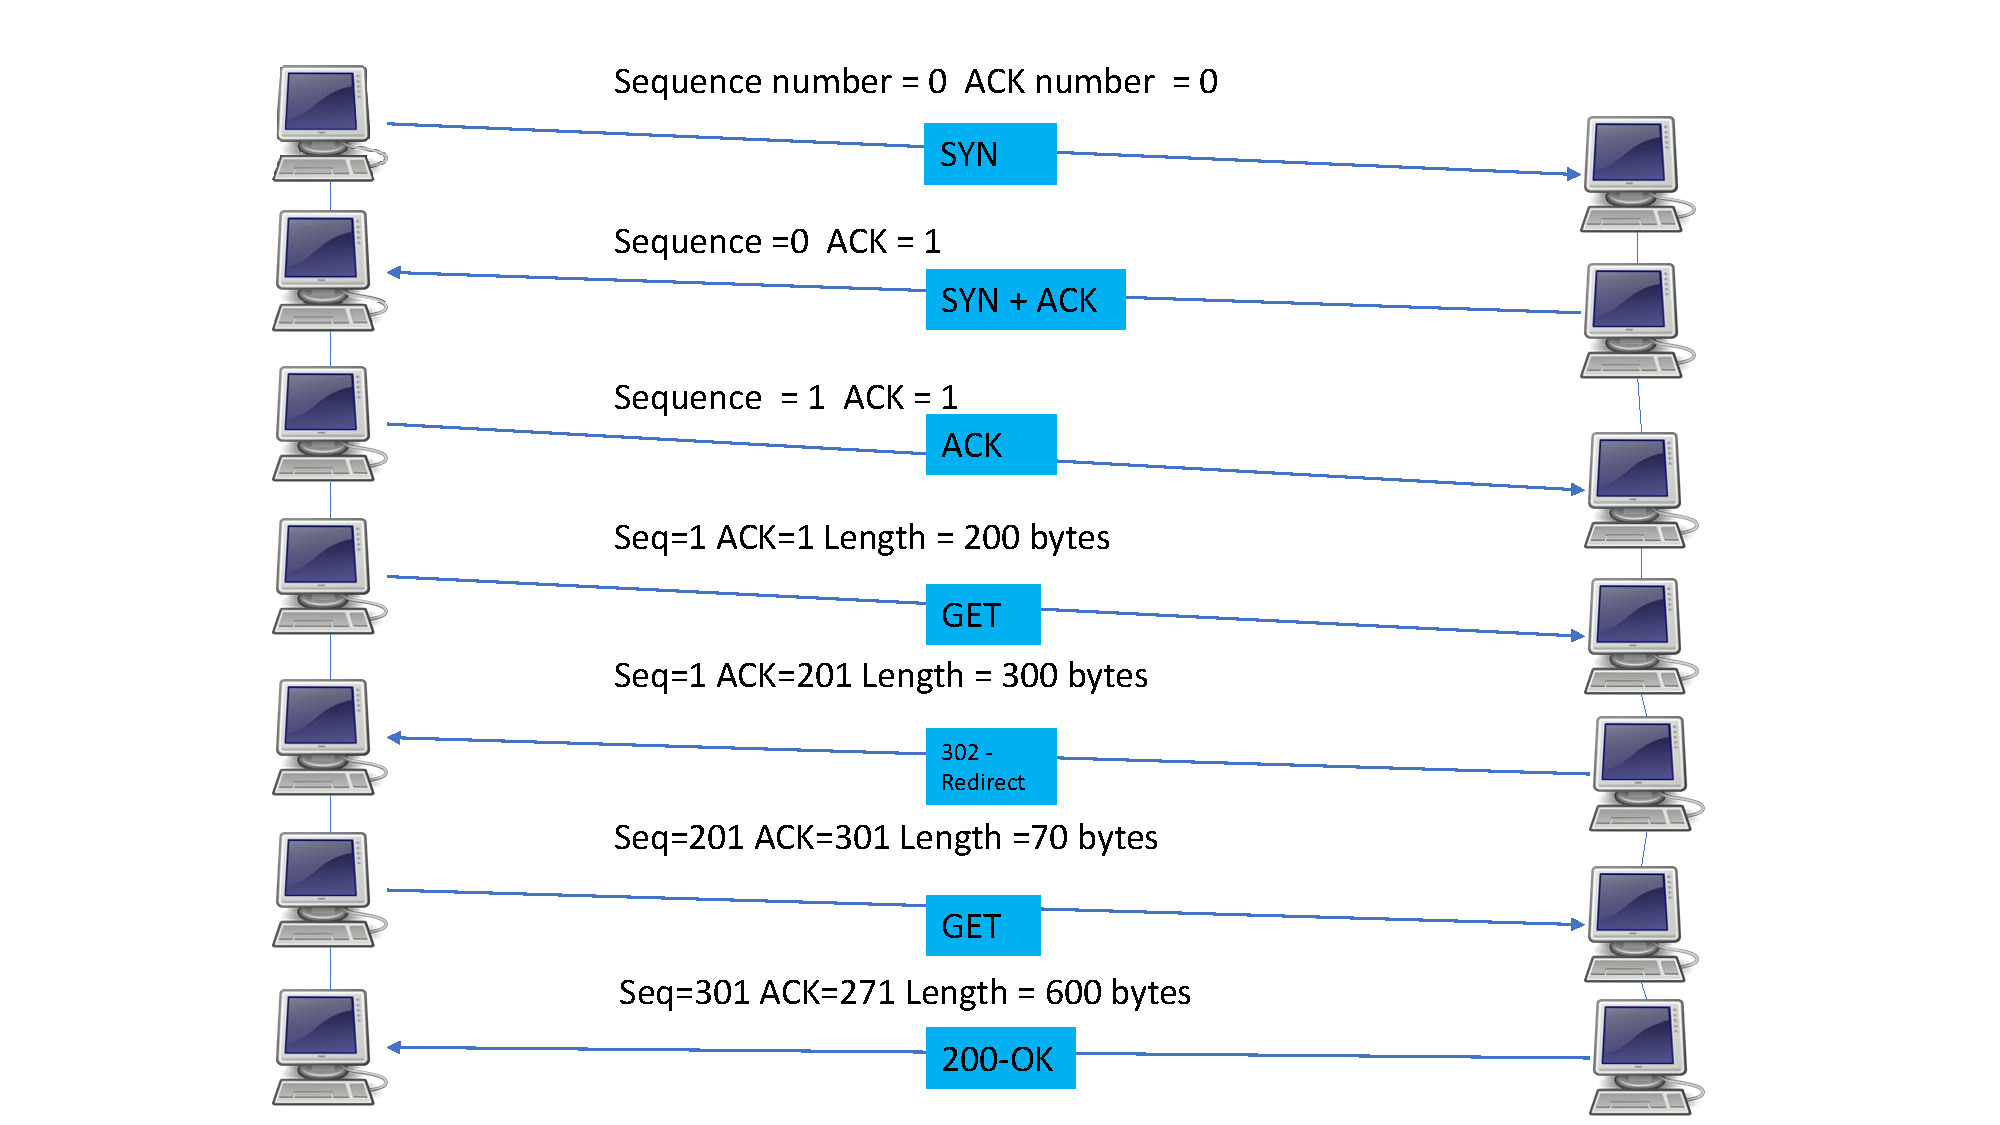
\includegraphics[width=0.87\textwidth]{ACK.pdf}
    \caption{TCP Relationship between SEQ and ACK where the response ACK = previous SEQ + Payload in bytes}
    \label{fig: TCP SEQ + ACK} 
\end{figure}

This completes this section on our methodology for development and implementation of our PEP. The next chapter will focus on our experimentation with the PEP in the University of Auckland Pacific Island Satellite Simulator. The chapter will report on the results found and will compare the findings with results found when PEPsal was tested on the Pacific Island Satellite Simulator by a Phd Student of University of Auckland. 
